%%% Dateikodierung: UTF-8
%%% äöüÄÖÜß  <-- keine deutschen Umlaute hier? UTF-faehigen Editor verwenden!

%%% Magic Comments zum Setzen der korrekten Parameter in kompatiblen IDEs
% !TeX encoding = utf8
% !TeX program = pdflatex 
% !TeX spellcheck = de_DE
% !BIB program = biber

\documentclass[master,english,smartquotes]{hgbthesis}
% Zulässige Optionen in [..]: 
%    Typ der Arbeit: 'diploma', 'master' (default), 'bachelor', 'internship' 
%    Hauptsprache: 'german' (default), 'english'
%    Option zur Umwandlung in typografische Anführungszeichen: 'smartquotes'
%    APA Zitierstil: 'apa'
%%%-----------------------------------------------------------------------------

\RequirePackage[utf8]{inputenc} % bei Verw. von lualatex oder xelatex entfernen!

\graphicspath{{images/}}  % Verzeichnis mit Bildern und Grafiken
\logofile{logo}           % Logo-Datei: images/logo.pdf (kein Logo: \logofile{})
\bibliography{references} % Biblatex-Literaturdatei (references.bib)

%%%-----------------------------------------------------------------------------
% Angaben für die Titelei (Titelseite, Erklärung etc.)
%%%-----------------------------------------------------------------------------

%%%\title{Peer to Peer File Sharing Netzwerke}
%%%\author{Andreas Zauner}
%%%\programname{Software Engineering}

%\programtype{Fachhochschul-Bachelorstudiengang} % auswählen/editieren
%%%\programtype{Fachhochschul-Bachelorstudiengang}

%%%\placeofstudy{Hagenberg}
%%%\dateofsubmission{2021}{07}{15} % {YYYY}{MM}{DD}

%%%\advisor{Alois B.~Treuer, Päd.\ Phil.} % optional

%\strictlicense % restriktive Lizenz anstatt Creative Commons (nicht empfohlen!)

%%%-----------------------------------------------------------------------------
\begin{document}
%%%-----------------------------------------------------------------------------

%%%-----------------------------------------------------------------------------
\frontmatter                                       % Titelei (röm. Seitenzahlen)
%%%-----------------------------------------------------------------------------
 
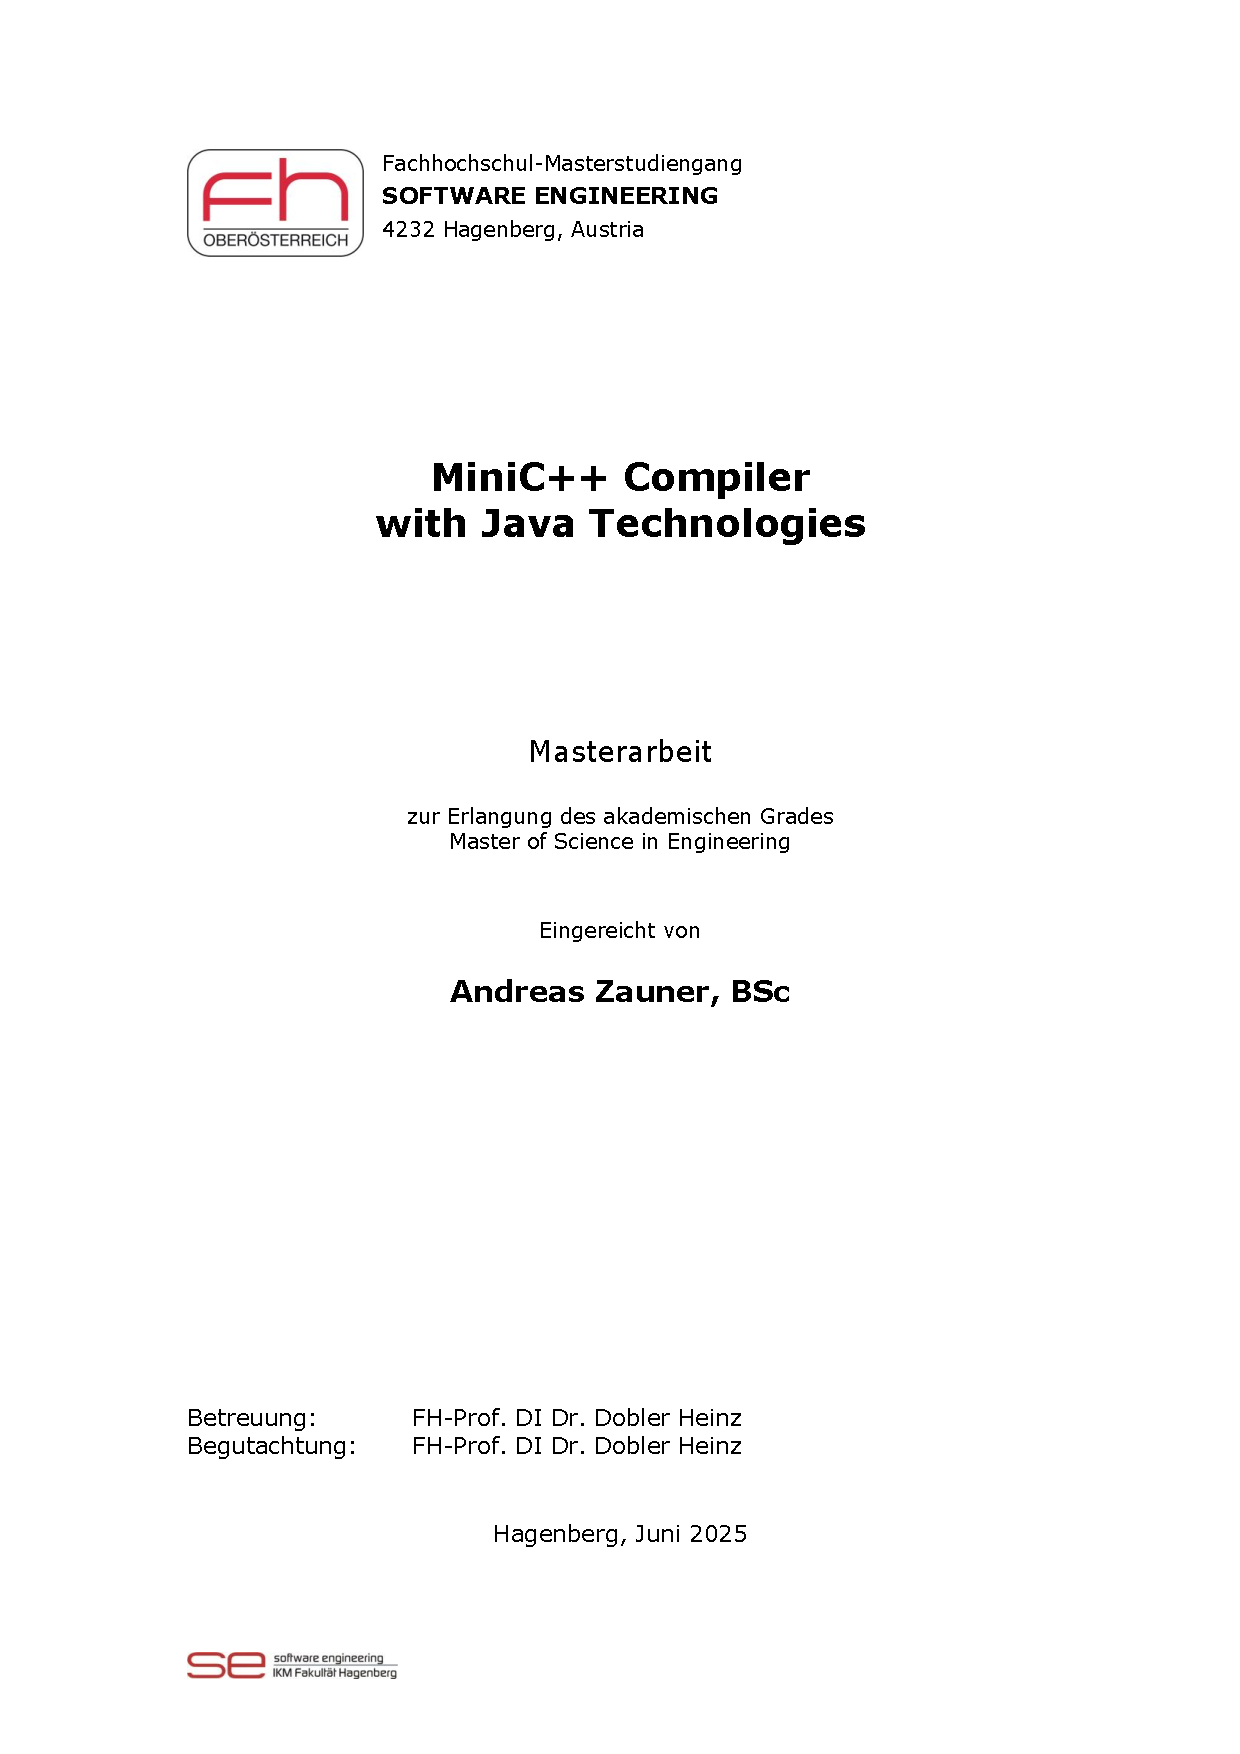
\includepdf[pages=1]{Titelblatt_Masterarbeit.pdf}
\includepdf[pages=2, pagecommand={\thispagestyle{plain}}]{Titelblatt_Masterarbeit.pdf}

\tableofcontents

\chapter{Kurzfassung}


\begin{german}

Diese Masterarbeit implementiert einen Compiler für MiniC\verb++| unter der Verwendung von Java-Technologien zur Erzeugung von Java-Bytecode. Für das Frontend wird der kombinierte Lexer- und Parsergenerator ANTLR verwendet, während das Backend die ObjectWeb ASM Bibliothek für die Bytecodegenerierung nutzt. Ähnlich zu Generatoren wie Coco-2 generiert ANTLR den Quellcode für einen Parser auf der Grundlage einer vorgegebenen Grammatik. ANTLR kann Code in mehreren Hostsprachen generieren; für diese Arbeit wurde Java gewählt. 

ANTLR ist ein Open-Source-Tool für die Spracherkennung. Es wurde erstmals 1992 veröffentlicht und wird seitdem von Terrence Parr kontinuierlich weiterentwickelt. In der aktuellen Version von ANTLR wird der adaptive-LL(*)oder ALL(*)-Parsing-Algorithmus verwendet. Dieser Algorithmus führt die Grammatikanalyse zur Parse-Zeit durch und überkommt dadurch die Einschränkungen früherer Versionen. ALL(*) erfordert nicht die Angabe einer maximalen Anzahl von Lookahead-Tokens. Stattdessen passt es sich an den aktuellen Kontext an und adaptiert die Anzahl der Lookahead-Token entsprechend.

Um einen abstrakten Syntaxbaum (AST) mit ANTLR zu erzeugen, werden drei Methoden unterstützt: Das Visitor-Pattern, das Listener-Pattern und die Verwendung einer attributierten Grammatik (ATG). Das Compiler-Frontend wird mit allen drei Methoden implementiert. Die drei Implementierungen werden in mehreren Aspekten verglichen und auf dieser Grundlage wird eine Empfehlung ausgesprochen.

ObjectWeb ASM ist eine in Java geschriebene Bibliothek zur Erzeugung von Java-Bytecode. Sie ist Open-Source und wird seit 2002 von Eric Bruneton entwickelt. Die Bibliothek wird in Compilern verwendet, die Java-Bytecode ausgeben, wie z.B. dem Kotlin-Compiler. Zur Generierung von Bytecode wird die auf dem Visitor-Pattern basierende API verwendet. 

Alle drei Frontend-Implementierungen sind mit dem Backend zu einer Anwendung verbunden, die Java-Bytecode aus MiniC\verb|++|-Code erzeugen kann. 

\end{german}
		
\chapter{Abstract}


\begin{english} %switch to English language rules
Peer-to-peer networks offer an alternative to the classic client-server model for exchanging data. In peer-to-peer networks, all clients communicate with each other. This means that the server, as the central element, can be omitted. This characteristic enables peer-to-peer networks to function even if individual participants in the network fail. In addition, peer-to-peer networks use the upload bandwidth of the individual clients, which is usually unused in traditional file sharing. 

This bachelor thesis deals in detail with peer-to-peer networks. First, known peer-to-peer networks are introduced and their characteristics are explained. Then it is shown where companies and organisations utilize peer-to-peer networks. A distinction is made between freely available networks and networks developed by companies themselves. Finally, a client for the BitTorrent network is developed. This client is able to exchange a file with other peers using the BitTorrent protocol. This shows how data exchange in a peer-to-peer network works on a technical level and which technologies are required for this.
\end{english}

			

%%%-----------------------------------------------------------------------------
\mainmatter                             % Hauptteil (ab hier arab. Seitenzahlen)
%%%-----------------------------------------------------------------------------

\chapter{Introduction}
\label{cha:introduction}

\section{Motivation}

Compilers are the backbone for computer programming. A compiler translates human-readable source code into something a computer can execute. This allows developers to focus on the functionality of the application, without having to worry about the technicalities of the concrete computer where the software will run on. For one programming language there may exist multiple compilers targeting different kinds of computers. This allows the same source code to run for example on Linux and Windows computers with Intel or ARM processors. This flexibility saves developers a lot of work, because they don't need to rewrite their application in the case they also want to target another operating system and/or processor. Furthermore, there exist compilers that target virtual machines like the Java Virtual Machine (JVM)\footnote{https://openjdk.org/groups/compiler/}. Generating code for a virtual machine has the advantage that there is no need for compilers for every target operating system and/or processor. Instead, for each operating system an implementation of the virtual machine is provided.

The process of compiling source code begins in the frontend of the compiler. The frontend reads the source code and constructs an abstract syntax tree (AST). The AST is a representation of the source code in memory. It contains only the necessary information that is needed to generate target code. The process of constructing the AST is based on the grammar of the programming language. Based on this grammar a lexer and parser are either written manually or get generated by a parser generator tool like ANTLR. In the case of ANTLR the generated lexer and parser by default construct a full parse tree from the input. From the parse tree an AST can be constructed using for example the visitor pattern. 

The AST functions then as the input for the backend of the compiler: The backend generates code for the target system. In the case of the JVM this is the so called bytecode.  APIs exist that provide an abstraction layer for the code generation. One API for bytecode generation is the open source project ObjectWeb ASM or just ASM \parencite{bruneton2007asm}. It provides an API that utilizes the visitor pattern to generate bytecode instructions. 


\section{Task and Goal}

MiniC++ is a subset of the C++ programming language. The scope of MiniC++ is very limited in comparison to C++. It is used at the University of Applied Sciences Upper Austria in Hagenberg for teaching software engineering master students about compilers in the formal languages class. In this class, all aspects of a compiler are discussed. First, the principles of lexers and parsers are explained. Then the concepts of syntax trees and further abstract syntax trees are introduced. Finally, code generation is explained. 

In the exercises, students use a MiniC++ compiler to compile MiniC++ source code to the .NET Common Intermediate Language (CIL). The frontend of the compiler is generated by using the compiler generator Coco-2 \parencite{doblerCoco2}. Which generates both, the lexer and the parser. There is only one input-file required for the definition of the lexer and the parser. Furthermore, attributes and semantic actions can be included to create an attributed grammar (ATG). 

In this master thesis, another compiler for MiniC++ will be created. This compiler will be built upon Java technologies. Output of the compiler will be Java bytecode that can be executed on the Java Virtual Machine (JVM). The frontend is based on a lexer and parser generated by the parser generator ANTLR\footnote{https://www.antlr.org/} (ANother Tool for Language Recognition). They are used to generate a full syntax tree. From this syntax tree an abstract syntax tree (AST) is constructed. The backend utilizes the ObjectWeb ASM\footnote{https://asm.ow2.io/} library. This library provides an API to generate Java bytecode. 

This master thesis will further explore the capabilities of ANTLR. ANTLR provides multiple ways to interact with the generated parser. The master thesis compares the advantages and disadvantages of each of these options.

\section{Theoretical Fundamentals}

This section explains the basic concepts of formal languages and how they are used in compilers. Furthermore, the individual components of a compiler are highlighted. 

\subsection{Formal Languages and Compilers}

Formal languages make up the fundament on which compilers are built upon. In comparison to natural languages, formal languages have a strict syntax which can be defined by a grammar. This grammar does not evolve naturally, as it does with natural languages. A formal grammar is defined by replacement rules. A replacement rule defines that a non-terminal symbol \textit{A} can be replaced by a sequence $\alpha$. The sequence may contain terminal and/or non-terminal symbols. 

Grammars can be classified according to the Chomsky hierarchy \parencite{CHOMSKY1959137}. Chomsky classifies formal languages and their grammars into four categories. Of those, the first two are relevant for compiler construction. Namely, regular grammars and context-free grammars. The four categories are differentiated by the type of rules that can be defined. The types of rules used then define which kind of automaton is needed to recognize sentences of the given language. 

\subsubsection{Regular Grammars}

Regular grammars make up the simplest group of grammars. For a grammar to be regular all rules must be in the form of $A\rightarrow a | a B$ or $S\rightarrow \epsilon$. This means that a non-terminal symbol $A$ can only be replaced by either a terminal symbol $a$ or a terminal symbol $a$ followed by a non-terminal symbol $B$. The only exception is the root rule $S$ which can be replaced by the empty sequence. 

To recognize a sentence of a regular grammar a finite automaton (FA) can be used. A deterministic FA (DFA) consists of the following elements:

\begin{itemize}
    \item $S$ finite, non-empty set of states,
    \item $\Sigma$ finite, non-empty set of symbols (alphabet),
    \item $s_0$ initial state, $s_0 \in S$,
    \item $\delta$ state transition function, $S \times \Sigma \rightarrow S$ and
    \item $F$ set of final states, $F \subseteq S$.
\end{itemize}

The DFA proceeds to read the symbols in $\Sigma$ one symbol at a time. The current symbol is then used in combination with the current state in the state transition function to acquire a new state. This process is continued until a final state is reached, meaning that a sentence has successfully been recognized. In case that for the current symbol and state no entry in the state transition function can be found, the recognition failed, and the given input is not a sentence of the language. 

A DFA can be implemented in a program to efficiently recognize sentences of a language. For more complicated regular languages nondeterministic finite automata (NFA) are easier to construct. A NFA program however is more complicated and slower compared to a DFA one. Every NFA can be transformed to a DFA to overcome this limitation. After transformation the constructed DFA may have more than the minimal number of states needed. A second transformation can be performed that reduces the DFA to a minimal DFA. 

\subsubsection{Context-Free Grammars}

Context-free grammars are the second group of grammars according to the Chomsky hierarchy. Context-free grammars include regular grammars, meaning that every regular grammar is also a context-free grammar. A replacement rule of a context-free grammar is in the form $A \rightarrow \beta$. Meaning that a non-terminal symbol $A$ can be replaced by a sequence $\beta$ containing terminal and/or non-terminal symbols or also $\varepsilon$, the empty sequence. 

In a context-free grammar central recursion is possible (direct or indirect). This allows the nested structures that are needed for programming languages, e.g., for expression hierarchies. Central recursion cannot be handled by a FA, for this a pushdown automaton (PDA) is needed. With a deterministic pushdown automaton (DPDA) all deterministic context-free grammars can be recognized. To recognize all context-free grammars a nondeterministic pushdown automaton (NPDA) is needed. For programming languages deterministic context-free grammars are used. 

There are two strategies for constructing a syntax tree from a sentence of a context-free grammar, namely top-down and bottom-up. Which strategy can be used depends on the kind of deterministic context-free grammar that is used. Following are the two most important conditions for context-free grammars:

\begin{itemize}
    \item \textbf{LL($k$) Condition:} Defines that a maximum of $k$ symbols look ahead are sufficient to deterministically decide on the next rule when using the \textit{top-down} strategy.
    \item \textbf{LR($k$) Condition:} Defines that a maximum of $k$ symbols look ahead are sufficient to deterministically decide on the next action(shift or reduce) when using the \textit{bottom-up} strategy.
\end{itemize}

The higher the value of $k$, the more complicated parsing becomes. Therefore, LL($1$) and LR($1$) grammars are preferred. For an LL($1$) or LR($1$) grammar only one symbol look ahead is needed for a deterministic decision. 

LL($k$) grammars can be recognized with a normal DPDA. For LL($1$) grammars it is also feasible to implement an efficient recursive descent parser. In the case of an LR($1$) grammar, the DPDA must be extended to be able to use an arbitrary amount of symbols on top of the stack. Only then is it able to recognize a sentence of an LR($1$) grammar with the \textit{bottom-up} strategy. It has to be noted that a DPDA which is able to recognize LR($k$) grammars, is also able to recognize LL($k$) grammars.

\subsection{Compiler Construction}

The task of a compiler is to translate code of a given source language into code of a target language. The source language being a human-readable programming language like Java and the target language being code for a given operating system and processor architecture, or a virtual machine. Compiling code can be separated into two main stages: frontend and backend.
The frontend executes of the following steps:
\begin{itemize}
    \item lexical analysis,
    \item syntactic analysis,
    \item semantic evaluation and
    \item intermediate language generation.
\end{itemize}

The backend performs optimization and code generation.

%\subsubsection{Lexical Analysis}
The lexical analysis is the first step of the compilation. It reads the source code and organizes it. The goal is to group individual characters into symbols and to skip meaningless characters (e.g., comments). The grammar of the source language provides the information about the symbols. This part of the grammar is defined using a regular grammar. 

The symbols can be divided into terminal symbols and terminal classes. Terminal symbols are special symbols like \texttt{=}, \texttt{(}, \texttt{-} and the keywords of the source language, e.g., \texttt{int}, \texttt{break},  \texttt{function}. Terminal classes are for example all numbers or identifiers. Comments are also handled at this step. Since comments usually have no influence on the generated code, they are removed. All recognized symbols are then passed to the parser (syntactic analysis and semantic evaluation). 


%\subsubsection{Syntactic Analysis}

The syntactic analysis takes the terminal symbols and classes recognized in the lexical analysis phase as input to construct the syntax tree. A context-free grammar provides the basis for the syntax tree. During the syntactic analysis the terminal symbols are grouped into syntactic elements according to the grammar. Furthermore, the syntactic integrity is also checked. In case that there is no grammar rule available for the current terminal symbol, the syntactic analysis fails, and a syntax error is reported.

%\subsubsection{Semantic Evaluation}

According to the principle of syntax-directed parsing, during the syntactic analysis the semantic evaluation is performed. This may include constructing the abstract syntax tree (AST). In the AST only the relevant information for the code generation is contained. For each rule in the grammar, there may be semantic actions associated with it, that get executed when the rule is visited. The semantic actions have access to the attributes of the rule. This information is used to generate the AST.  

%Taking the AST as a basis, the intermediate language code generation is performed. This includes for example generating the symbol table. 

Afterwards, the intermediate language code is analyzed and optimized. This may include optimizations such as inlining or loop unrolling. Depending on the use case, more aggressive optimizations can also be performed. 

Finally, the code generation unit takes the optimized code and generates the appropriate instructions for the target language. 
\chapter{Methods and Tools for Compiler Frontends}

In this chapter  methods and tools for the construction of compiler frontends are explained. This explanation is focused on the parser generator ANTLR. The basis for this chapter is the book "The Definitive ANTLR 4 Reference" by \textcite{Antlr4Reference}.

\section{Attributed Grammars}

Parser generators like ANTLR or Coco-2 require the definition of the grammar of the source language in a specific format. These formats also allow for the declaration of attributes and semantic actions in the grammar. Semantic actions have access to the attributes of symbols (terminal and non-terminal) of a rule. Some symbols have attributes associated with them. The combination of a grammar, attributes and semantic actions is called an attributed grammar.  


There are two types of attributes: inherited and synthesized attributes. The former ones are computed based on the attributes of the parent node. Synthesized attributes are based on the attributes of the children nodes.  
The type of attributes available depends on the parsing strategy. For a top-down strategy the attributes of child-nodes are not available, as they have not been parsed yet. Conversely, when using the bottom-up strategy, the attributes of parent nodes are not available. 

Especially relevant are the attributes of terminal classes. Through the attribute of a terminal class like \texttt{number}, the actual number that this class node holds can be accessed. These kinds of attributes are provided by the lexical analyzer. 

In listing \ref{lst:Coco2ATG} a simple attributed grammar for Coco-2 for arithmetic expressions is shown. This grammar uses semantic actions to calculate the result of an arithmetic expression. Semantic actions are encoded inside \lstinline{SEM<< >>} blocks; in this case C\verb|#| code. Synthesized attributes provide the results of the calculations from the child nodes. These attributes are available inside the semantic actions where the actual calculation is performed. 

While it is convenient to embed semantic actions directly into the grammar, it is not without disadvantages. By embedding code of a specific language, it is no longer possible to use the same grammar to generate a parser in another implementation language. Parser generators like ANTLR provide multiple implementation languages to generate a parser for. 

\begin{GenericCode}[float,numbers=none,caption=Attributed Grammar for Coco-2 for simple arithmetic expressions., label=lst:Coco2ATG]
Expr<<out int e>> =    LOCAL<<int t = 0; e = 0;>>
  Term<<out e>>             
  { '+' Term<<out t>>    SEM<<e = e + t;>>
  | '-' Term<<out t>>    SEM<<e = e - t;>>
  }.

Term<<out int t>> =    LOCAL<<int f = 0; t = 0;>>
  Fact<<out t>>
  { '*' Fact<<out f>>  SEM<<t = t * f;>>
  | '/' Fact<<out f>>  SEM<<t = t / f;>>
  }.
  
Fact<<out int f>> =    LOCAL <<f = 0;>>
    number<<out f>>
  | '(' Expr<<out f>> ')'.

\end{GenericCode}

\section{ANTLR}

In this section, the parser generator ANTLR (ANother Tool for Language Recognition) is explained. First, a general overview of the history of ANTLR is given, followed by the introduction of the parsing algorithm currently employed by ANTLR, namely ALL(*). Finally, the general functionality of ANTLR is explained.  

\subsection{History}

"ANTLR (ANother Tool for Language Recognition) is a powerful parser generator for reading, processing, executing, or translating structured text or binary files". As the acronym of ANTLR states, it is a tool for language recognition. ANTLR was first released in 1992 and has since then been in continuous development. The original creator and maintainer of the project is Terence Parr. ANTLR is written in Java and is open sourced under the BSD license. Its source code can be viewed on GitHub\footnote{https://github.com/antlr/antlr4}. 

Many projects utilize ANTLR. Notable examples include the Java Object-Relational Mapping tool \cite{HibernateWeb2024} and the NoSQL database Apache \textcite{Cassandra2024}.

ANTLR originally started of as the master thesis of Terrence Parr \parencite{PCCTSHistory1994}. A first alpha release was created in 1990, that only generated LL(1) parsers. Version 1 of ANTLR incorporated the new parsing algorithm developed by Parr that allowed to create parsers for LL(k) grammars \parencite{parrPhd1993}. Version 2 then provided incremental improvements.   

Version 3, released in 2006 introduced a new parsing algorithm called LL(*) \parencite{LLSParsing2011}. The LL(*) parsing strategy performs parsing decisions at parse-time with a dynamic lookahead. The number of lookahead tokens increases to an arbitrary amount and decreases again using backtracking. However, the maximum amount of $k$ lookahead tokens still needs to be specified. Version 3 also introduced ANTLRWorks\footnote{https://www.antlr3.org/works}, a graphical IDE for the construction of ANTLR grammars.

The current version 4, released in 2013 again introduced a new parsing algorithm adaptive-LL(*) or ALL(*). The most significant improvement of ALL(*) over LL(*) is that the maximum number of lookahead tokens no longer needs to be specified. ANTLR v4 added support for the visitor and listener patterns\footnote{https://github.com/antlr/antlr4/blob/dev/doc/listeners.md}, enabling easier interaction with the syntax tree. 

\subsection{Parsing Algorithm Adaptive-LL(*)}
\label{sec:allstar}

The Adaptive-LL(*) or ALL(*) parsing strategy is introduced in the paper "Adaptive LL(*) parsing: the power of dynamic analysis" by \textcite{ALLParsing2014} and is the basis for this section. This parsing algorithm is used  for ANTLR version 4. As the title suggests, ALL(*) performs the analysis of the grammar at parse time. 

\subsubsection{Limitations of LL(*) Parsing Algorithm}

To understand the need for ALL(*), it is necessary to highlight why the previous strategy LL(*) is insufficient. LL(*), introduced by \textcite{parr2011ll}, was developed as an improvement to the existing general LL (GLL) \parencite{GLL2010} and general LR (GLR) \parencite{tomita1991generalized} parsers. For ambiguous grammars these parsers return multiple parse trees, which are undesirable for parsers of programming languages. GLL and GLR are  designed for natural languages, which are inherently ambiguous. LL(*) overcomes these limitations by using regular expressions that are stored inside a deterministic finite automaton (DFA) to offer mostly deterministic parsing. Using the DFA allows for regular lookahead even though the grammar itself is context-free. 

However, the LL(*) grammar condition cannot be checked statically, leading to the case that sometimes no regular expression is found that distinguishes the possible productions. Such situations are detected by the static analysis and then backtracking is used instead. Backtracking however comes with the disadvantage that for rules in the format $A \rightarrow a | ab$, the second alternative will never be matched, since backtracking always chooses the first alternative. 

\subsubsection{Dynamic Grammar Analysis with ALL(*)}

With ANTLR version 4 the parsing strategy Adaptive-LL(*) or ALL(*) was introduced. The main difference to ANTLR version 3 is that the grammar analysis is now performed at parse-time, and is no longer static. This overcomes the limitations of the static analysis LL(*) performs and enables the generation of correct parsers for context-free grammars. The only exception are grammars that contain indirect or hidden left-recursion\footnote{Indirect left-recursion is a rule like $A \rightarrow Bx, B \rightarrow Ay$. $\epsilon$ productions cause hidden left-recursion. Take a rule $B \rightarrow \epsilon$ that produces only the empty chain $\epsilon$ and another rule $A \rightarrow BA$. Since B's only production is to $\epsilon$ the second rule causes a left-recursion. }. From an engineering perspective it was seen to be too much effort, since these grammars are deemed to be not common. Direct left-recursion is possible, because ANTLR rewrites the grammar to be non-direct left-recursive before passing it to the ALL(*) parsing algorithm. 

At a decision point (a rule containing multiple alternatives), ALL(*) starts a subparser for each alternative in pseudo-parallel. A subparser tries to match the remaining input to the selected alternative. If the input does not match, the subparser dies off. All subparsers process one symbol at the time in pseudo-parallel. This guarantees that the correct alternative can be found with minimum lookahead. In the case of ambiguity due to multiple subparsers reaching the end of file or coalescing, the first alternative will be chosen. 

The performance of ALL(*) is improved by employing a cache. This cache is implemented in the form of a DFA. The DFA stores the same information as the DFA generated by LL(*) from static analysis. After a lookahead, the DFA stores which production resulted from the lookahead phrase. If at a later time the same lookahead phrase is being processed, the correct production can be retrieved from the DFA. Theoretically, a DFA is not able to recognize a context-free grammar, however due to the analysis being performed at parse time, the analysis only needs to be performed on the remaining input. Since the remaining input is a subset of the context making it regular. Another optimization is the usage of a graph-structured stack (GSS). The GSS makes sure that during the prediction, no computation is performed twice, effectively acting as a cache. 

%In some cases it is necessary for ALL(*) to examine the parse stack to make a decision. 
%section about SLL
The theoretical runtime complexity of ALL(*) is $O(n^4)$. This stems from the fact that in the worst case the ALL(*) parser needs to make a prediction for each symbol and each launched subparser then needs to inspect the entire remaining input. In practice ALL(*) performs linearly for common programming languages like Java or C\verb|#|.


\subsection{Functionality}

ANTLR generates a combined lexer and parser from a single grammar file. The generated parser is a recursive descent parser. ANTLR supports various implementation languages such as Java, C\verb|#| or C++. The syntax used by the ANTLR grammar supports extended BNF (EBNF) operators such as \texttt{?}. To interact with the generated parser, ANTLR optionally generates interfaces and implementations for the listener and visitor pattern.

ALL(*) does not use a separate lexical analysis phase. Instead lexical and syntactical analysis are integrated into a unified process. Lexical rules are treated as parser rules, therefore a separate lexical analysis phase is not needed. Since the phases are combined, it is possible for ALL(*) to perform context-sensitive lexing. The lexer can make a decision based on the current parsing context. The parsing is directly performed on the raw input stream and not on a separate token stream. 

\subsubsection{Semantic Predicates}

ANTLR supports the definition of so-called \textit{semantic predicates}. Semantic predicates are boolean expressions, defined in the host language that allow for the dynamic alteration of the language generated by the grammar. If a semantic predicate is present for a production, the production can only be accepted if the semantic predicate evaluates to true. Semantic predicates are expressed inside \verb|{ }| parenthesis followed by $?$. Listing \ref{lst:ANTLRSemPred} illustrates an example use case of a semantic predicate. The rule \texttt{blockEnd} contains a semantic predicate specifying that the production can only be accepted if there is currently a block on the stack. 

A semantic predicate also has access to the current token. This enables conditions that directly interact with the input. For example separate productions for even and uneven numbers could be used. The semantic predicate then checks if the number is even or not.  


\subsubsection{Semantic Actions}

In ANTLR grammars semantic actions can be defined. Semantic actions can be inserted in every parser rule, before, in between and after symbols. Similar to semantic predicates, the semantic action is to be defined in the implementation language. Semantic actions are defined inside \verb|{ }| parenthesis. To access a symbol the name of the symbol prefixed by \verb|$| can be used. In Listing \ref{lst:ANTLRSemPred} semantic actions are used in the \texttt{blockStart} \texttt{blockEnd} rules. For the \texttt{blockEnd} it has to be noted that semantic predicates and actions can be used together. 

% semantic actions

\begin{AntlrCode}[float,numbers=none,caption=Example grammar using a semantic predicate and a semantic action., label=lst:ANTLRSemPred]
grammar Example;
@members {
    java.util.Stack<String> blockStack = new java.util.Stack<>();
}

program: statement* EOF;

statement
    : blockStart
    | blockEnd
    | otherStatement
    ;

blockStart: 'begin' { blockStack.push("block"); };

blockEnd: 'end' { !blockStack.isEmpty() }? { blockStack.pop(); };

otherStatement: 'print' IDENTIFIER;

IDENTIFIER: [a-zA-Z_][a-zA-Z_0-9]*;

WS  : [ \t\r\n]+ -> skip;
\end{AntlrCode}


\subsubsection{Alternative Labels for Rule Alternatives}

Per default ANTLR generates one method for each rule. In the case of multiple alternatives for a rule, the handling of the alternatives would need to be done manually. Therefore, ANTLR offers the possibility to attach a label to each of the alternatives. Then a method for each alternative will be generated separately. One use case is highlighted in listing \ref{lst:ANTLRRuleAlt}. The rule \texttt{type} matches to either one of the four types. Each alternative has a label associated to it by using \verb|#| as the prefix for the alternative name. With this definition four methods will be generated corresponding to each of the alternatives as explained above.     

\begin{AntlrCode}[float,numbers=none,caption=Example rule using alternative labels for the rule alternatives., label=lst:ANTLRRuleAlt]
  type
      : 'int'     #IntType
      | 'bool'    #BoolType
      | 'long'    #LongType
      | 'string'  #StringType
      ;
\end{AntlrCode}

\section{Syntax Tree and Abstract Syntax Tree (AST)}

A syntax tree is a hierarchical representation of the syntactical structure of a sentence. Also referred to as a parse tree, this representation is usually generated by a parser. A syntax tree contains the information of the entire sentence based on the grammar of that language. Each inner node in the syntax tree corresponds to a rule in the grammar. The leaf nodes represent terminal symbols and inner nodes are non-terminal symbols. Concatenating the leaf nodes from left to right of the syntax tree results in the original sentence from which the syntax tree was constructed from. 

Listing \ref{lst:SyntaxTreeEx} shows the syntax tree of the arithmetic expression \texttt{5 * 3 + 7} based on the grammar in \ref{lst:Coco2ATG}. 
%TODO
This syntax tree contains the non-terminal symbol \texttt{Expression, Term, Fact} and the terminal class \texttt{number}. The expression is built from two terms and one operator. The left term represents a multiplication consisting of two factors and an operator. All factors in the syntax tree contain the terminal class \texttt{number} which hold the concrete numbers. This structure further enables the representation of the precedence rules of arithmetic operations directly in the syntax tree.  

\subsection{Abstract Syntax Tree (AST)}
In an abstract syntax tree (AST) only a subset of the nodes from the original syntax tree are included. The goal is to focus on the semantic aspects of the syntax tree. Syntactical details, e.g., semicolons are omitted. 

The generation of an AST from a syntax tree can be done in multiple ways. One method is to generate the AST during the parse, which increases performance since the syntax tree does not need to be traversed twice. This can be implemented by using an attributed grammar with semantic actions that embed the AST generation code directly into the parser. Parsers like ANTLR also support the listener pattern to execute code during the parse. Alternatively the AST can be generated after the parse phase from the syntax tree. To traverse the syntax tree the visitor pattern can be used for example.  

The AST is then used in the subsequent stages of a compiler. This transformation is performed to create a new tree which omits all information that is of no importance to the following stages of the compiler. Subsequent code optimization may further slim down the AST. 

Continuing with the previous example, listing \ref{lst:ASTEx} shows the AST of the arithmetic expression \texttt{5 * 3 + 7}. This AST still contains the same semantic meaning as the full syntax tree, however it needs fewer nodes for that. Instead of using the non-terminal symbols, the operator is used, effectively encoding the same information. In this example, the node count can be reduced from 14 to 5.

\begin{GenericCode}[float,numbers=none,caption=Syntax tree of the arithmetic expression \texttt{5 * 3 + 7} based on the grammar in listing \ref{lst:Coco2ATG}., label=lst:SyntaxTreeEx]
                                       Expr   
                                   /    |    \
                                Term    +    Term
                              /   |   \        |    
                           Fact   *   Fact    Fact  
                            |          |       |
                          number     number  number
                            |          |       |
                            5          3       7
\end{GenericCode}

\begin{GenericCode}[float,numbers=none,caption=Abstract syntax tree of the arithmetic expression \texttt{5 * 3 + 7}., label=lst:ASTEx]
                                      +
                                    /   \
                                   *     7
                                 /   \
                                3     5
\end{GenericCode}

\section{Visitor-Pattern for Tree Transformation}

In the case that a syntax tree is already present, the visitor-pattern can be used to create an AST from the syntax tree. Using the visitor-pattern, the syntax tree gets traversed and then step by step the AST is constructed. The visitor-pattern allows for the separation of algorithms from the objects they operate on. Instead of including the code for the generation of an AST object in the syntax tree object, a separate object, a so-called \textit{visitor} is taking care of this. 

To implement visitor-pattern for a syntax tree, the best approach is to use interfaces or abstract classes for the nodes of the syntax tree and the visitors. Listing \ref{lst:ListPatIntEx} shows a possible implementation for an interface and abstract class in Kotlin. This code is based on the syntax tree shown in listing \ref{lst:SyntaxTreeEx}. Each class of the syntax tree implements the  abstract class \texttt{SyntaxTreeNode}. For the visitor class the \texttt{SyntaxTreeVisitor} interface needs to be implemented. Both classes are generic. This allows the implementation of the visitor to use an arbitrary type as a return value. Multiple visitors can then be implemented using the generics, so that each visitor can return one type of the AST types. In this case it is helpful to create an abstract base visitor that provides an empty implementation for all interface's methods. Then the concrete visitor only needs to override the methods that are relevant for the specific AST type.  

A \texttt{SyntaxTreeNode} can then be visited by calling its \texttt{accept} method. Inside the \texttt{accept} method, the appropriate method of the \texttt{SyntaxTreeVisitor} will be called. As can be seen in listing \ref{lst:ListPatNumbNode} the \texttt{NumberNode} calls the \texttt{visitNumberNode} with itself as the parameter. This behavior is analogous for all other nodes of the syntax tree. 


\begin{KotlinCode}[float,numbers=none,caption=Interface and abstract class used to implement the visitor-pattern., label=lst:ListPatIntEx]
sealed class SyntaxTreeNode {
    abstract fun <T> accept(visitor: SyntaxTreeVisitor<T>): T
}

interface SyntaxTreeVisitor<T> {
    fun visitNumberNode(node: NumberNode): T
    fun visitOperatorNode(node: OperatorNode): T
}
\end{KotlinCode}


\begin{KotlinCode}[float,numbers=none,caption=Implementation of the \texttt{NumberNode} class inheriting from the \texttt{SyntaxTreeNode}., label=lst:ListPatNumbNode]
  data class NumberNode(val value: Int) : SyntaxTreeNode() {
    override fun <T> accept(visitor: SyntaxTreeVisitor<T>): <T> {
        return visitor.visitNumberNode(this)
    }
}
  \end{KotlinCode}


\section{Listener-Pattern for Tree Transformation}

The listener-pattern is used for \textit{listening} to events or notifications from another object. In the context of parsing, the listener-pattern is used to handle parse events coming from the parser. This includes events such as entering and exiting a node during the parse. When using the listener-pattern the parse tree is only traversed once. This is because the events get pushed to the listeners during the parse. 

To implement the listener-pattern for the construction of an AST, a listener interface is needed. The listener interface contains method declarations for entering and exiting each node type. The methods take the syntax tree node as the input parameter. A possible implementation for the listener interface is shown in.  In case of the \textit{enter} methods, the symbols for the syntax tree node have not been parsed yet, so no data from them is available yet.

A concrete listener will then implement the interface and register/subscribe itself to the events of the parser. When the parser enters or exits a node during parse it will call the respective method with the parsed syntax tree node for all listeners. 

\begin{KotlinCode}[float,numbers=none,caption=Implementation of the \texttt{ExpressionListener} interface., label=lst:ListPatExprList]
interface ExpressionListener {
    fun enterExpr(node: Expression)
    fun exitExpr(node: Expression)

    fun enterNumer(number: Number)
    fun exitNumber(number: Number)
}
  \end{KotlinCode}


\chapter{Java Virtual Machine (JVM)}

This chapter focuses on the Java Virtual Machine (JVM). First the foundation and history of the JVM will be explained. Further focus is put on JVM itself and its functionality. In the following section the language of the JVM \textit{bytecode} is introduced. Finally, the bytecode manipulation tool ObjectWeb ASM is highlighted. This chapter is based on the specification of the JVM provided by \textcite{JVMHistoryOracle}.

\section{History}

 As the name suggests, the Java Virtual Machine is the virtual machine used to execute java programs. In 1994 Sun Microsystems Inc. developed the JVM because of their requirement for Java to be platform and operating system independent. By using a virtual machine as an intermediary, Sun was able to move the multiplatform aspect away from the compiler. 

One of the original use cases for Java and therefore the JVM was embedding of so-called applets in browsers. Applets were used in addition to the HTML document format, which at that time only provided limited functionality. Similar to HTML the applets were platform independent, which eased the development for the website creators. The first browser incorporating applets was HotJava. 

Java was originally closed source, however in 2006 Sun Microsystems Inc. began work on open sourcing the Java compiler and the JVM under the OpenJDK project \parencite{SunOpenSourceJava}. On November 13, 2006 the JVM implementation developed by Sun called HotSpot was open sourced under the GPL license.

The Version of the JVM specification is tied to the Java Version, but for the \texttt{class} files a separate version number so-called \textit{class file format version} is used. For the initial JDK release 1.0 the class file format version 45 was used. 

Various companies and organizations provide implementations of the JVM. For example GraalVM is an implementation of the JVM with the ability to perform ahead-of-time (AOT) compilation for a Java program. While this increases the performance of the application, it can only be executed on the platform it was compiled for. Another example is picoJava, which is a processor specification with the goal of enabling native execution of bytecode for embedded systems \parencite{PicoJava}. \textcite{PicoJavaFPGA} presented an implementation of picoJava on an FPGA.
%pico java




\section{Architecture}

The basic task of the JVM is to read a \texttt{class} file and execute the bytecode instructions contained in it. The specification defines only the abstract machine. How the bytecode is executed on the actual physical processor, or what optimizations are to be performed, is up to the implementer of the JVM specification. An official reference implementation of the JVM called OpenJDK\footnote{https://openjdk.org/} is provided by Oracle. 
The JVM architecture can be seen in figure \ref{fig:JVMArchitecture}. It consists of the following elements: 

\begin{itemize}
    \item \textbf{Class Loader}: Loads \texttt{class} files into memory.
    \item \textbf{Runtime Data Area}: Manages all runtime memory used in the JVM.
    \item \textbf{Execution Engine}: Executes bytecode instructions.
    \item \textbf{Native Method Interface}: Interfaces with the native host system. 
\end{itemize}

\begin{figure}[]
    \centering
    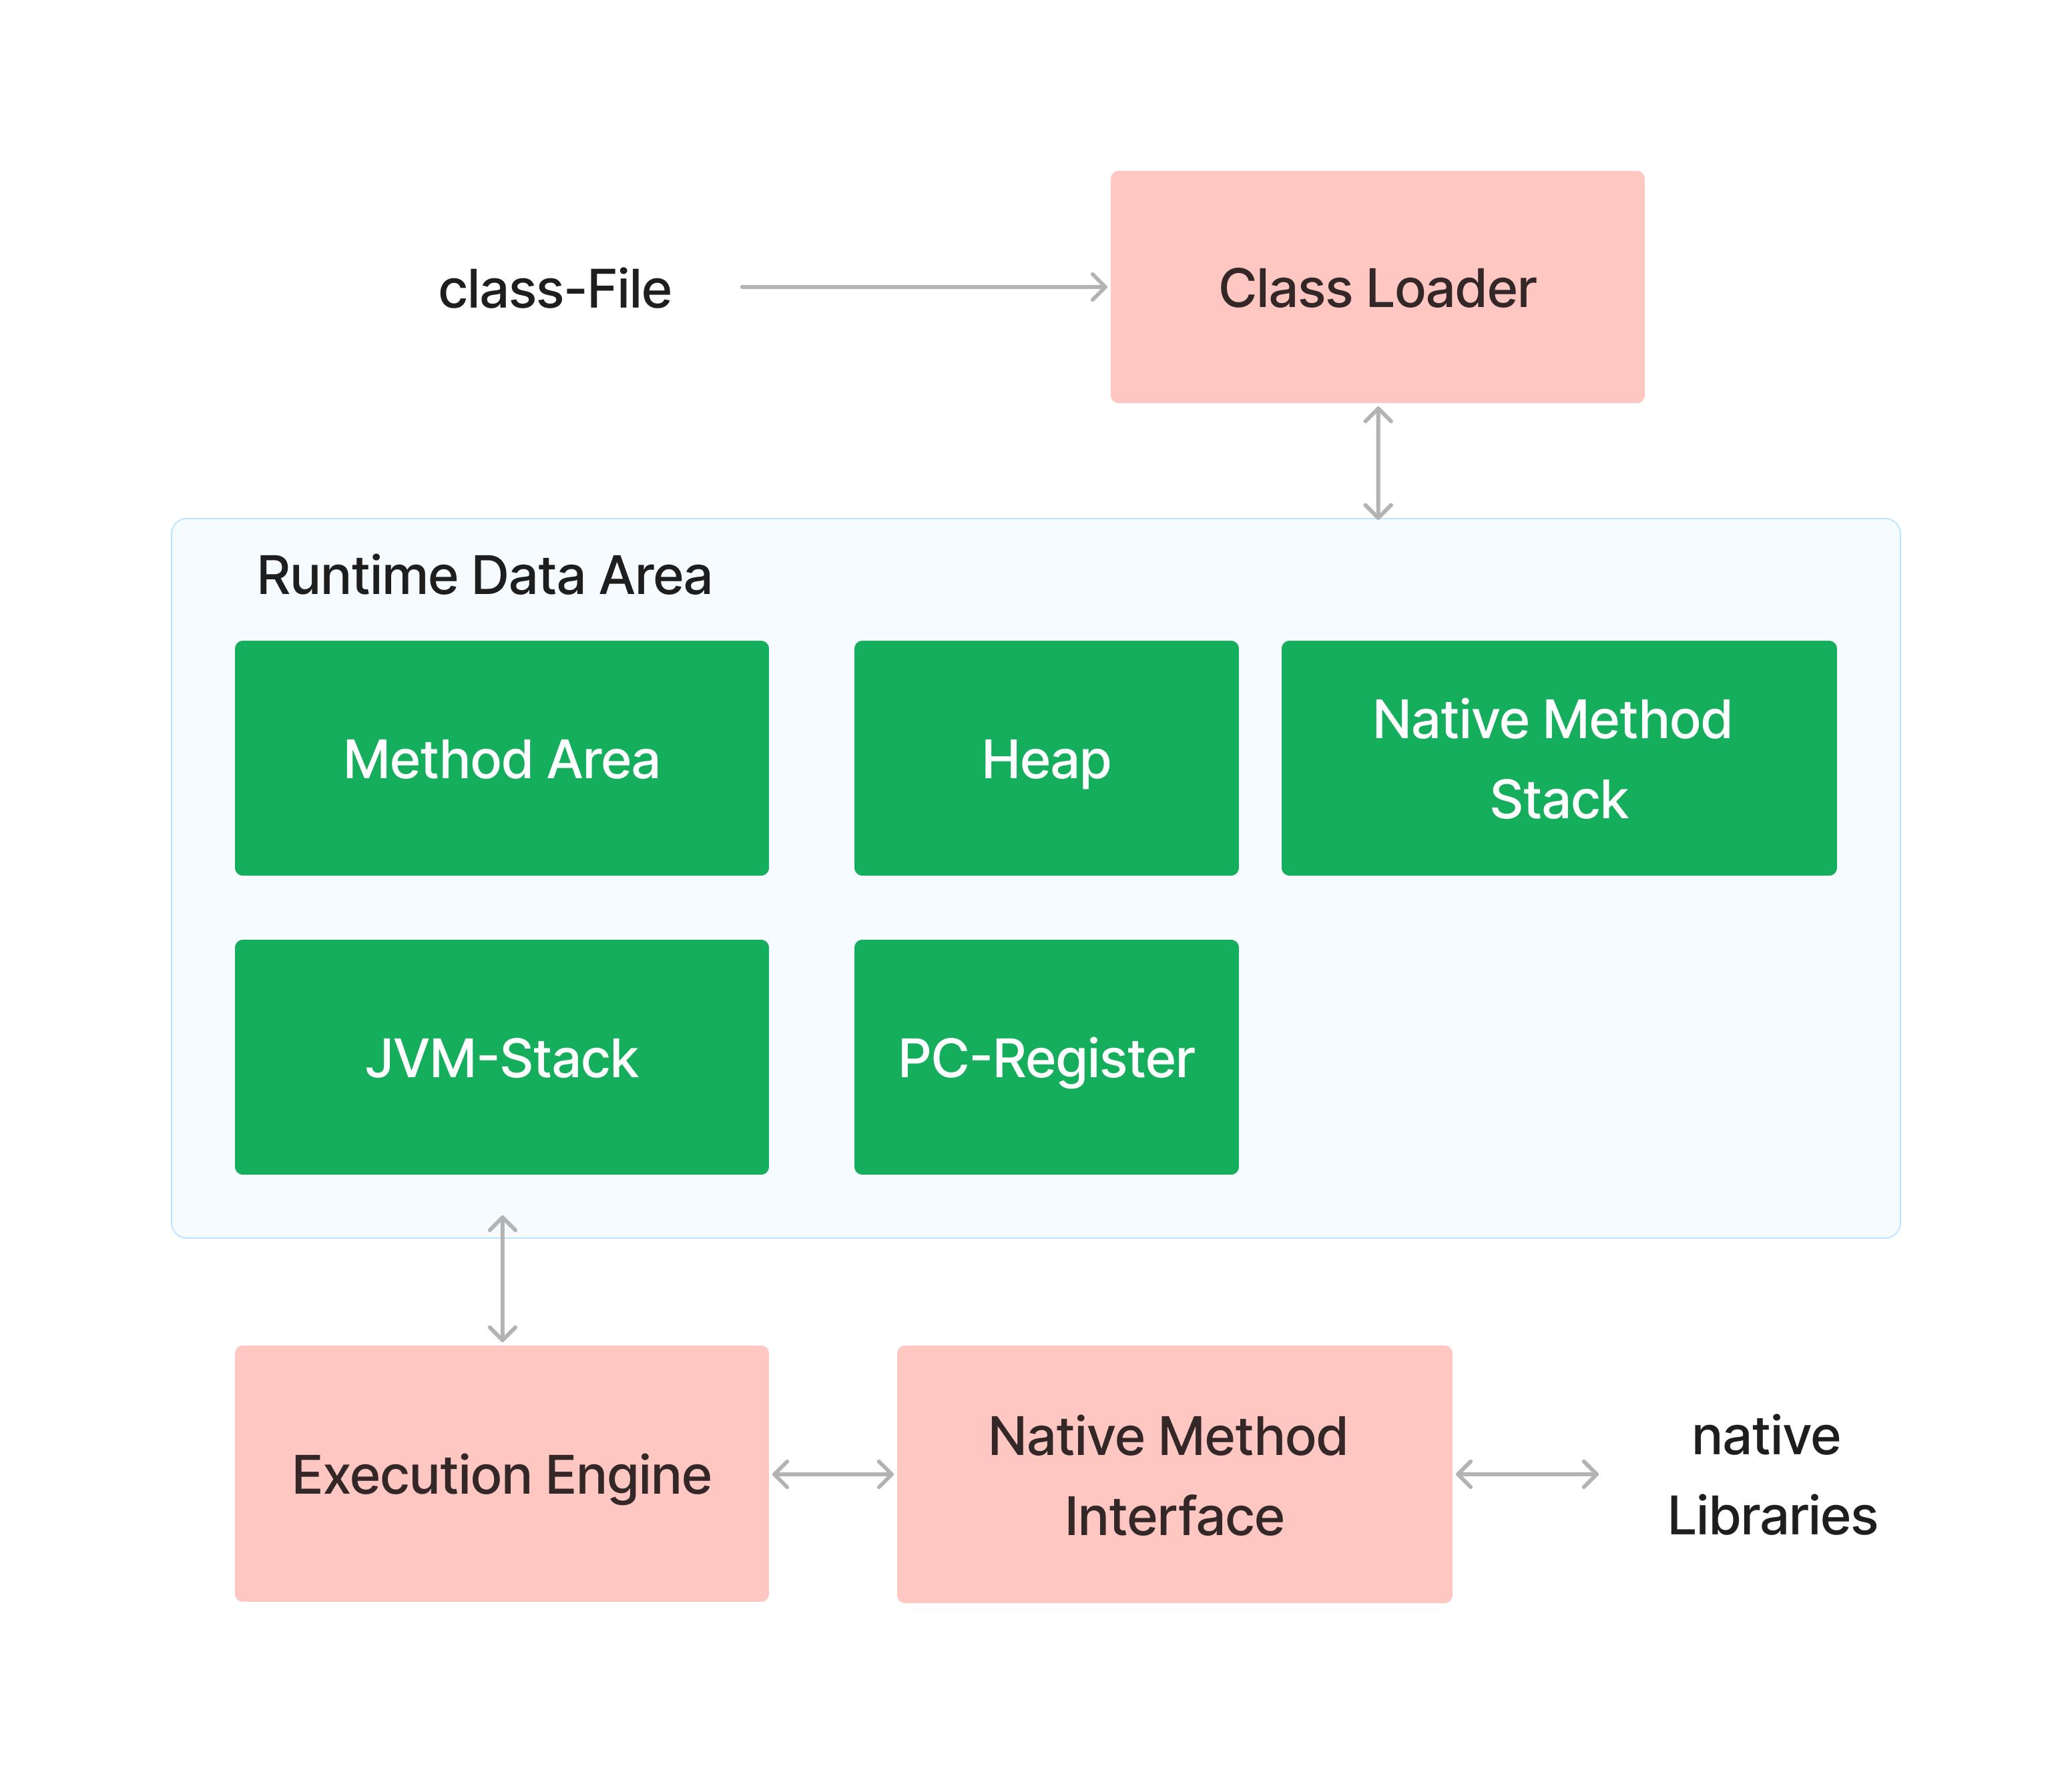
\includegraphics[width=\textwidth]{JVM_Architecture.png}
    \caption{Architecture of the JVM.}
    \label{fig:JVMArchitecture}
\end{figure}

\subsection{\texttt{class} File Format}

A \texttt{class} file contains the necessary information that is needed to execute a program on the JVM. One \texttt{class} file contains the definition of either a single class, interface or module. A \texttt{class} file is structured as follows: 

\begin{itemize}
    \item Magic Number
    \item Version Info
    \item Constant Pool
    \item Access Flags
    \item This Class
    \item Super Class
    \item Interfaces
    \item Fields
    \item Methods
    \item Attributes
\end{itemize}

At the beginning of the \texttt{class} file is the magic number. It is responsible for identifying a \texttt{class} file. The magic number is the same for every \texttt{class} file. Next is the version of the \texttt{class} file format. The JVM uses the version to determine if the \texttt{class} file is compatible with it.

The \textit{constant pool} acts as a storage for all constants and symbolic references contained in the file. For example the reference to a method or a string literal. An entry in the constant pool consists of a tag which specifies one of 17 constant types, followed by information describing the constant. Depending on the type, the length of the constant may change. A string literal for example would require more memory than an integer. 

The \textit{access flag} entry is a flag mask that defines the permissions and properties of the class or interface. Possible flags include for example, whether the class is \texttt{public, final, abstract} or not. 

The \textit{this class} entry contains the name of the current class in the form of an index to an entry in the constant pool. Analogous the \textit{super class} entry defines the name of the superclass of this class. In case that the class does not inherit from a superclass, the index is zero. The following section lists all implemented interfaces, again as a list of indexes in the constant pool. 

In the \textit{fields} section all member fields of the class are listed. Each field description consists of four elements: Access flags, similar to the class level access flags, e.g., \texttt{public, private}. An index to the name of the field in the constant pool. An index to the descriptor (type specification) of the field in the constant pool. Finally, the entry can have optional attributes associated with it, e.g., the constant value (for static fields). An entry in the \textit{methods} section contains the same values, only the descriptor is used to describe the method signature (parameter and return type).

Finally, in the \textit{attributes} section, additional metadata of the class is stored. Most importantly, this section contains the bytecode for each method of the class. Other information includes for example, a list of exceptions thrown by each method, the name of the source file or a mapping from bytecode instructions to source code line numbers.

\subsection{Class Loader}

The class loader takes care of loading bytecode into the JVM memory. There are three tiers of class loaders:

\begin{itemize}
    \item \textbf{Bootstrap}: Loads JDK internal classes and core libraries. Implemented in native code and not accessible by an application. 
    \item \textbf{Extension}: Loads extensions of the standard Java classes from the JDK extensions directory. 
    \item \textbf{Application}: Loads all application level classes. These are located via the classpath. Classes can be put on the classpath by using an environment variable or command line option. 
\end{itemize}

The class loaders are organized in a parent-child hierarchy. The Bootstrap class loader is the parent of the Extension class loader, which itself is the parent of the Application class loader. When a request is made to load a \texttt{class} file, the class loader first delegates the request to its parent class loader. Only if the parent class loader cannot locate the class the current class loader will attempt to load it. This process is performed so that no two class loaders attempt to load the same class. The loading process is separated into three stages. Loading, linking and initialization.

In the loading stage the bytecode is loaded into the JVM. The bytecode can be loaded from a file, the network or another source. The bytecode is loaded into the JVM as a \texttt{Class} object.

In the second stage linking is performed. This stage is separated into the three substages verification, preparation and resolution. Verification is performed to ensure that the loaded bytecode adheres to the JVM's rules. Rules include such as requiring that a return instruction must match its method's return type, or that a \texttt{throw} instruction must only throw values that are instances or subclasses of \texttt{Throwable}. Verification is performed because the JVM must guarantee that only correct \texttt{class} files are executed and no exploitation through malicious bytecode is taking place. The second substage preparation creates the static fields of a class or interface and allocates the memory needed for them. The static fields further are assigned their respective default values. Explicit initializers are executed during initialization, during preparation no bytecode is executed. Resolution then resolves all symbolic references inside the class. Symbolic references are used for example when referencing another class or interface. For each symbolic reference resolution determines a concrete value. 

If linking has been successful the class or interface is initialized. Explicit initializer of static fields are executed as are static initializer blocks of the class or interface.

\subsection{Runtime Data Areas}

The runtime data areas of the JVM are regions of memory used during the execution of a program. Each memory area serves a specific use case. Some memory areas are specific to a thread. They get created when a thread is created and cleaned up on thread termination. Others are alive for the entire duration of the JVM's runtime.  

\subsubsection{PC Register}

The \texttt{program counter} or PC register is the memory area which contains the bytecode instruction that is currently being executed. Each thread inside the JVM has its own PC register. In the case that a native method is executed, the PC register's value is undefined.

\subsubsection{JVM Stacks}

A JVM Stack is a thread-specific memory area that is created in tandem with the thread. A stack in the JVM is similar to a stack in languages such as C. An instance of a stack stores \textit{frames} for method-calls. On method invocation a new frame is created. Conversely, when the method invocation is finished, the frame is destroyed. 

A frame contains information related to a single method invocation. This includes the following:

\begin{itemize}
    \item Local variables and method parameters
    \item Operand stack
    \item Reference to constant pool of the method's class
    \item Return address 
\end{itemize}

The operand stack is used for intermediate calculations and storing results from other method invocations. The reference to the constant pool is needed to resolve the targets for method calls and field accesses. The return address stores the address of the calling method. Once the method invocation has completed control will be returned to this address.

\subsubsection{Heap}

In the \textit{heap} all object instances and arrays are stored. The heap is shared across all threads and is created on JVM startup. Contrary to programming languages like C, it is not possible in the JVM to manually reclaim/free the memory allocated by an object or array. Instead, the JVM utilizes an automatic storage management system known as a \textit{garbage collector}. The garbage collector automatically reclaims memory from objects and arrays that are no longer referenced by any other object or variable in the program. The JVM specification does not require a specific garbage collector algorithm, rather the implementer can choose which algorithm to use or also allow the user to select the algorithm. While the garbage collector automatically reclaims memory, it is also possible to manually request a cleanup through an API. There is however no requirement for the garbage collector to honor this request, so it may be ignored. 

\subsubsection{Method Area}

The method area is a section of the memory that is available to all threads inside the JVM and is created on JVM startup. It stores metadata of the classes loaded into the JVM. This includes the runtime constant pool, field and method data and the bytecode for methods and constructors.

\subsubsection{Native Method Stacks}

Similar to JVM stacks \textit{native method} stacks are associated with a method invocation and store information relevant to that invocation. However, in this case the invoked method is executed natively on the host system. Instead of bytecode, native code, written in e.g. C, is executed. The native method stack serves as an interface between the native code and the bytecode inside the JVM.  
  
\subsection{Execution Engine}

The JVM's execution engine is responsible for executing the bytecode contained in the loaded \texttt{class} files. It takes bytecode instructions and transforms them into something the host system can execute. This may be through interpretation or just-in-time (JIT) compilation. The JVM specification does not specify how the bytecode is executed on the host system. Therefore, in this section the execution engine \textit{HotSpot} of the JVM reference implementation \textcite{OpenJDKHotspotRuntime} is explained.

The HotSpot execution engine consists of two main parts: The interpreter and the JIT-Compiler. For memory management the execution engine is supported by the garbage collector, that automatically reclaims memory from unused objects and arrays. The java native interface (JNI) enables the JVM to call and execute code and libraries written in other languages like C or C\verb|++|.

\subsubsection{Interpreter}

The interpreter reads bytecode instructions sequentially and translates them to target code the host system can execute. This allows the JVM to start executing bytecode right away, without having to wait for any JIT compilation to be performed. In comparison, .NETs' Common Language Runtime (CLR) performs a JIT compilation of a methods' code as soon as it is first invoked\parencite{MicrosoftCILToNative}. 

HotSpot uses a template-based interpreter. On JVM startup HotSpot creates an interpreter based on the data in the so called \texttt{TemplateTable}. The \texttt{TemplateTable} contains information on the assembly code corresponding to each bytecode instruction. A template in this case is a description of a bytecode. The generated templates are specific to the host operating system and architecture. The interpreter fetches the template corresponding to the current bytecode instruction and executes it. The template is fetched by using an accessor function provided by the \texttt{TemplateTable}. This approach leads to higher performance than using a switch-statement, which may have to compare the current instruction with all cases to find the correct code to execute. A downside of this approach is the need for extra platform and operating system specific code needed for the dynamic code generation. Some operations, like a lookup in the constant pool, are still performed via the JVM runtime, since they are too complicated to be implemented in assembly code directly. 

Initially, all code on the JVM is interpreted. The runtime performs adaptive optimization by monitoring the code execution for methods that are executed often, so-called \textit{hotspots}. For those hotspots the runtime performs optimization. Specifically a method detected as a hotspot will be just-in-time compiled, so that it can be natively executed on the host system. 

\subsubsection{Just-In-Time Compilation (JIT)}

To increase performance, the JVM runtime employs just-in-time (JIT) compilation. Contrary to ahead-of-time compilation, which translates the code before the execution, JIT compilation translates the code during the execution of the program. Because the compilation is performed while the program is executing, considerations need to be made about the performance implication of the compilation. Therefore, the JVM uses a two stage tiered compilation: The C1 or \textit{client} compiler and the C2 or \textit{server} compiler.

%https://cr.openjdk.org/~vlivanov/talks/2015_JIT_Overview.pdf

Through profiling the JVM runtime identifies hotspots, also referred to as \textit{hot methods}. These are methods that are executed often. Methods that are only called rarely are referred to as \textit{cold methods}. The JIT compiler focuses only on hot methods for multiple reasons: Compiling bytecode to native code takes up processor time that cannot be used for the actual execution of the program. Furthermore, the compiled code needs to be stored in memory and thus completely compiling bigger programs to native code make take up a significant amount of memory. Only compiling hot methods strikes a balance between performance and memory consumption. Also, empirically programs spend most of their execution time on a small amount of the entire codebase. 

Once a method has been identified for compilation, the first JIT compiler C1 compiles the method to native code. The C1 compiler prioritizes compilation speed and therefore only performs basic optimizations. After compilation the methods' body is replaced by the compiled code, leading to the method being executed natively and no longer interpreted. During compilation code used for profiling is also added. The profiling information is used for the second stage of the JIT compilation. 

When a method that was compiled with C1 passes an execution threshold, the C2 compiler will compile the method again. This time the focus is on performing aggressive optimizations for maximum performance, which consumes more times than the first compilation. The C2 compiler uses the information gained through profiling to perform optimizations that lead to the best performance. This may include optimization techniques such as loop unrolling or inlining. The C2 compiler does not add any code for profiling which further improves performance. In some cases the assumptions that the C2 compiler made based on the profiling data can turn out to be wrong, which in turn can lead to the method being returned to the C1 compilation level.

\subsubsection{Java Native Interface (JNI)}


\begin{JavaCode}[float,numbers=none,caption=Declaration of a native method in Java., label=lst:JNINativeMethod]
    public class Example {
        public native void nativeMethod();
    }
\end{JavaCode}


The Java Native Interface (JNI) is an API that enables the code executed inside the JVM to interoperate with applications and libraries that are written in other languages. This API is necessary because there are cases when the entirety of the application cannot be implemented inside the JVM. For example there might be libraries only available in C/C++, but not for the JVM. The JNI then allows calling those libraries from within the JVM. Listing \ref{lst:JNINativeMethod} shows the declaration of a native method in Java. The \texttt{native} keyword signalizes to the JVM that the implementation of the method will be provided in native code.


The JNI makes it possible to create, inspect and update JVM objects. For that the JNI provides a type mapping between the JVM types and native equivalents. Further, methods located inside the JVM can be called or exceptions thrown from within native code.

Using the JNI inside an application however limits the number of systems it can be executed on. The native part of the application needs to be compiled for every architecture and operating system the application is intended to run on. Native methods manually manage the memory they have allocated and therefore programming errors can lead to memory leaks within the application.  

\section{Bytecode}

Bytecode is the instruction set of the JVM. It serves as an intermediate language between high level languages such as Java or Kotlin, and low level languages such as assembly which can be natively executed on a CPU. High level languages only need to target bytecode to be cross-platform. As long as a JVM implementation is present for a given architecture and operating system, the bytecode can be executed without needing to be compiled again. 

\subsection{Structure}

In terms of code execution JVM is organized as a stack machine with registers. Each method being executed is structured as a frame containing an operand stack and local variables, which can be seen as registers. The operand stack and number of variables inside a frame are each able to contain up to 65535 entries.

A bytecode instruction is structured as a one byte long opcode followed by zero or more one byte long operands. The maximum possible number of opcodes is therefore 256. Most of them are in use, while some are reserved for internal and future use. Each instruction has a mnemonic associated with it. Instructions that can operate on multiple types are prefixed by the concrete type they are operating on. For example the instruction for adding together two integers is known by the mnemonic \texttt{iadd}. The following types are supported in bytecode:

\begin{itemize}
    \item \texttt{boolean}
    \item \texttt{byte}
    \item \texttt{char}
    \item \texttt{short}
    \item \texttt{int}
    \item \texttt{float}
    \item \texttt{reference}
    \item \texttt{returnAddress}
    \item \texttt{long}
    \item \texttt{double}
\end{itemize}

Most instructions for the types \texttt{byte}, \texttt{char} and \texttt{short} and all for \texttt{boolean} are internally converted to \texttt{int}, therefore in these cases the \texttt{int} based instructions are used instead.

The \texttt{reference} type is analogous to pointer types in languages like C. It is type-safe and managed by the JVM. The JVM also keeps track of the references for garbage collection purposes. If there are no references anymore pointing to an object, the garbage collector can reclaim the memory it occupied. The \texttt{returnAddress} type represents pointers to opcodes of JVM instructions. This type is only used internally and is not accessible otherwise.


\subsection{Categories of Instructions}

The instructions in the bytecode instruction set can be categorized depending on their functionality. Instructions from each category work together to perform more complex actions. 

\subsubsection{Load and Store Instructions}

Load and store instructions allow the loading of values onto the operand stack and storing values from it into variables. These instructions function within the frame of a method. Load instructions like \texttt{iload} or \texttt{aload} load an integer or array respectively onto the operand stack. To load a constant onto the operand stack instructions like \texttt{bipush} and \texttt{ldc} can be used. \texttt{ldc} loads a constant from the constant pool of the class while \texttt{bipush} takes one operand (the constant value), that is loaded onto the operand stack. When a value from the operand stack is to be stored into a variable instructions like \texttt{istore} or \texttt{astore} are available. 

\subsubsection{Arithmetic Instructions}

Arithmetic instructions perform calculations using the values on the operand stack. The result of the calculation is then put on the operand stack. There are separate instructions for integer and floating point calculations, e.g. \texttt{iadd} and \texttt{fadd} for integer and floating point additions respectively. In the case of an over or underflow no exception is thrown. The bytecode instruction set further includes instructions for bitwise logical operations like AND (\texttt{iand}). 

\subsubsection{Type Conversion Instructions}

Type conversion instructions make it possible to change the type of a numeric value. They can be used to perform an explicit conversion. The JVM supports widening conversions (e.g. from \texttt{int} to \texttt{long}; \texttt{i2l}) and narrowing conversions (e.g. from \texttt{float} to \texttt{int}; \texttt{f2i}). For some conversions there may be a loss of information. Widening conversions like from \texttt{int} to \texttt{float} can lose some of the least significant bits of the source value. 

\subsubsection{Object related Instructions}

The bytecode instruction set contains separate instructions for class instances and arrays, even though they are both considered as objects by the JVM. To create a class instance the instruction \texttt{new} is used, while for an array \texttt{newarray} is used. To access class fields the \texttt{getfield} instruction can be used for instance variables and \texttt{getstatic} for class variables. When loading an entry from an array there is a separate instruction for each type, e.g. \texttt{iaload} for loading an integer from an array. For storing a value inside a class instance or array analogous instructions are available. 

\subsubsection{Operand Stack Management Instructions}

In some cases it is beneficial to perform manipulations on the operand stack directly. For example to implement peephole optimization, it is necessary to duplicate a value on the operand stack as an alternative to loading a variable two times\parencite{mckeeman1965peephole}. The instruction for that is \texttt{dup}. The instruction set further provides instructions like \texttt{pop} or \texttt{swap}. 

\subsection{Sample program}
\chapter{Implementation Frontend}

This chapter explains the implementation of the frontend of the compiler. First the additional technologies that are used in the development of the frontend are listed. Then the AST and symboltable are explained. In the following section the ANTLR grammar is shown. Based on this grammar three implementations for the AST transformation are explained: Visitor-pattern, listener-pattern and via an attributed grammar. 

\section{Used Technologies}

In this section the additional technologies used for the development of the frontend are explained. This includes chosen the programming language and the additional libraries used.

\subsection{Kotlin}

For the implementation the programming language Kotlin is chosen. Kotlin can be compiled to bytecode, which makes it possible to use Java libraries in Kotlin code. Kotlin has advantages over Java in some aspects. For example, null safety\footnote{https://kotlinlang.org/docs/null-safety.html} is implemented into the language via explicit nullability within it's type system. This requires the caller of a field to explicitly handle nullable fields and thus reduces the risk of a null reference exception. 

\subsection{AspectJ}

The compiler frontend utilizes AspectJ in it's handling of semantic errors. AspectJ is a library that enables aspect oriented programming in Java. Aspect oriented programming makes it possible to handle cross-cutting concerns in a central place without having to modify code in other areas. It can be used for compile time and runtime weaving of cross-cutting concerns. In the compiler frontend, runtime weaving using annotations is used.  

\subsection{ANTLR Preview Plugin}

During development with the JetBrains IntelliJ IDE, the ANTLR preview plugin\footnote{https://plugins.jetbrains.com/plugin/7358-antlr-v4} is used. The plugin developed by the ANTLR creator Terrance Parr, offers various features that enhance the process of creating and working with ANTLR. When developing an ANTLR grammar, syntax highlighting and checking for syntactic and semantic errors is provided. The included navigation window inside the IDE further enables testing of the grammar, without having to generate the combined lexer and parser manually first. To generate the combined lexer and parser the plugin includes a tool window which includes common configuration settings.

\section{ANTLR Grammar}

The ANTLR grammar is based on the MiniC++ grammar in EBNF-form. This grammar is transformed into the ANTLR grammar syntax. ANTLR grammars are stored inside \texttt{.g4} files. Each rule inside the grammar is delimited by a semicolon. 

\subsection{Header Section}

At the top of the grammar file, the name of the grammar is specified. In this case \texttt{minicpp}. In this section options can also be specified, like the implementation language of the lexer and parser or the package/namespace of the generated code. These and other options can also be specified via command line options during the generation. In this case the necessary options are specified in the tool window of the ANTLR preview plugin. 

%if in need add picture of tool window

\subsection{Terminal Classes and Comments}

The grammar contains three terminal classes shown in listing \ref{lst:ANTLRMiniCppTermClass}. The \texttt{IDENT} terminal class is used for all identifiers and requires them to start with a letter followed by an arbitrary number of letters and digits. For integer number the \texttt{INT} terminal class specifies a sequence of one or more digits. Signs are handled in the parser rules. Strings are defined as a sequence of characters starting and ending with double quotes. All characters except the special characters for line end are allowed. The comment and whitespace handling is performed by the \texttt{WS}, \verb|LINE_COMMENT| and \verb|BLOCK_COMMENT| lexical rules. These are special rules that when matched tell the parser to skip them and therefore not include them in the syntax tree. 

\begin{AntlrCode}[float,numbers=none,caption=Terminal classes of the MiniC++ ANTLR grammar., label=lst:ANTLRMiniCppTermClass]
IDENT:          [a-zA-Z_][a-zA-Z_0-9]*;
INT:            [0-9]+;
STRING:         '"' (~[\r\n"] | '""')* '"';
WS:             [ \t\n\r]+ -> skip;
LINE_COMMENT:   '//' ~[\r\n]* -> skip;
BLOCK_COMMENT:  '/*' .*? '*/' -> skip;
\end{AntlrCode}


\subsection{Root}

The top rules of the grammar are shown in listing \ref{lst:ANTLRMiniCppTop}. The root rule \texttt{miniCpp} contains zero or more elements of the rule \texttt{miniCppEntry} followed by the lexical rule \texttt{EOF}. \texttt{EOF} is a default lexical rule provided by ANTLR signaling the end of the file. \texttt{miniCppEntry} defines the elements that can be used at the top level of the miniC\verb|++| source file. These are variable and constant definitions and function declarations and definitions. \texttt{SEM} is the lexical rule defining a semicolon. 

\begin{AntlrCode}[float,numbers=none,caption=Top rules of the MiniC++ ANTLR grammar., label=lst:ANTLRMiniCppTop]
miniCpp:     (miniCppEntry)* EOF;
miniCppEntry:     constDef
                | varDef
                | funcDecl
                | funcDef
                | SEM
                ;
\end{AntlrCode}



\subsection{Variables and Constants}

Listing \ref{lst:ANTLRMiniCppVarConstDef} shows the parser rules variable and constant definitions. Both definitions can have multiple entries, which are separated by a comma. In the case of a constant definition entry, the initialization value is required. For a variable this is optional. The \texttt{STAR} optional lexical rule classifies a field as an array if present. The \texttt{initOption} parser rule consists of three production alternatives specifying the possible initialization values. 

\begin{AntlrCode}[float,numbers=none,caption=Variable and constant defintions of the MiniC++ ANTLR grammar., label=lst:ANTLRMiniCppVarConstDef]
constDef:        CONST type constDefEntry (COMMA constDefEntry)* SEM ;
constDefEntry:   IDENT init ;

varDef:          type varDefEntry (COMMA varDefEntry)* SEM ;
varDefEntry:     STAR? IDENT (init)? ;

init:            EQUAL  initOption ;
initOption:      BOOLEAN      #BooleanInit
               | NULLPTR      #NullptrInit
               | (SIGN)? INT  #IntInit
               ;
\end{AntlrCode}

\subsection{Function Declaration and Definition}

The rules for a function declaration and definition are shown in listing \ref{lst:ANTLRMiniCppFuncDeclDef}. In MiniC\verb|++| to call a function there must be at least a declaration of the function further ahead in the source code. Function declarations and definitions both start with the function head that consists of the return type, identifier and an optional parameter list. In the case of a function definition, the function head is followed the \texttt{block} rule, which contains the method's body. 

The parameter list can consist either of a single entry, the \texttt{void} type, or of one or more actual input parameters. Each parameter specified by the \texttt{formParListEntry} rule, consists of a type, an optional star and brackets indicating an array followed by the identifier of the parameter.


\begin{AntlrCode}[float,numbers=none,caption=Function declaration and defintion of the MiniC++ ANTLR grammar., label=lst:ANTLRMiniCppFuncDeclDef]
funcDecl:         funcHead SEM;
funcDef:          funcHead block;
funcHead:         type STAR? IDENT LPAREN formParList? RPAREN;
formParList:      (     VOID
                  |     formParListEntry (COMMA formParListEntry)*
                  );
formParListEntry: type STAR? IDENT (BRACKETS)?;
\end{AntlrCode}

\subsection{Statements}

The parser rule defining a statement is shown in listing \ref{lst:ANTLRMiniCppStatAlt}. The statement rules serves as a container for all concrete statement types. For example, the \texttt{ifStat} rule can be seen in listing \ref{lst:ANTLRMiniCppStatIf}. It consists of the \texttt{if} keyword followed by the condition in parentheses and a statement which should be executed if the condition is met. Optionally an else statement can be specified. This rule does not suffer from the \textit{dangling else} problem. In such cases ANTLR resolves the ambiguity by always choosing the first successful production. 

\begin{AntlrCode}[float,numbers=none,caption=Statement rule and it's production alternatives of the MiniC++ ANTLR grammar., label=lst:ANTLRMiniCppStatAlt]
stat:  ( emptyStat  | breakStat
       | blockStat  | exprStat
       | ifStat     | whileStat
       | inputStat  | outputStat
       | deleteStat | returnStat
       );
\end{AntlrCode}

\begin{AntlrCode}[float,numbers=none,caption=If Statement rule  of the MiniC++ ANTLR grammar., label=lst:ANTLRMiniCppStatIf]
ifStat:      'if' LPAREN expr RPAREN stat elseStat?;
elseStat:    'else' stat;
\end{AntlrCode}



\subsection{Expressions}

Part of the grammar for expressions is shown in listing \ref{lst:ANTLRMiniCppExprBool}. At the top of every expression is an \texttt{orExpr} followed by zero or more \texttt{exprEntry} elements. In case an \texttt{exprEntry} is present, the expression performs one or mor assignments. Each \texttt{exprEntry} consists of an assignment operator signalizing the type of assignment, and an \texttt{orExpr} that provides the value to be assigned. The \verb|orExpr| and \verb|andExpr| rules implement their respective boolean operators. The \verb|relExpr| rule consists of a \verb|simpleExpr| and zero or more \verb|relExprEntry| elements. The \verb|relExprEntry| rule handles relative expressions with the \verb|relExprOperator| rule, which contains the relative operators like greater or less than. The \verb|simpleExpr| rule begins with an optional sign that is relevant for integer values, followed by a term and zero or more \verb|simpleExprEntry| elements. The \verb|simpleExprEntry| rule consists of a sign followed by a term. The precedence rules for arithmetic operations are realized inside the grammar.



\begin{AntlrCode}[float,numbers=none,caption=Expression rules for assignment and boolean operations of the MiniC++ ANTLR grammar., label=lst:ANTLRMiniCppExprBool]
expr:                 orExpr (exprEntry)*;
exprEntry:            exprAssign orExpr;
exprAssign:           EQUAL      #EqualAssign
                    | ADD_ASSIGN #AddAssign
                    | SUB_ASSIGN #SubAssign
                    | MUL_ASSIGN #MulAssign
                    | DIV_ASSIGN #DivAssign
                    | MOD_ASSIGN #ModAssign
                    ;
orExpr:             andExpr ( '||' andExpr )*;
andExpr:            relExpr ( '&&' relExpr )*;
relExpr:            simpleExpr
                    ( relExprEntry )*;
relExprEntry:       relOperator simpleExpr;
simpleExpr:         (SIGN)?
                    term ( simpleExprEntry )*;
simpleExprEntry:    SIGN term;
\end{AntlrCode}

The rules for terms and factors are shown in listing \ref{lst:ANTLRMiniCppExprTermFact}. A term consists of a fact, which contains an optional negation making it a \verb|notFact|, followed by zero or more \verb|termEntry| elements. The \verb|termEntry| rule realizes multiplication, division and modulo operations via the \verb|termOperator| rule. The \verb|fact| rule contains six possible productions. Three types of value literals can be used as a factor: integer, boolean or null-pointer. Another option is the array initialization, defined by the \verb|#NewArrayFact| alternative. The \verb|#ExprFact| alternative allows for precedence using an expression contained in parentheses. To read the value of a variable or array, or call a function the \verb|#CallFact| alternative using the \verb|callFactEntry| rule is used. The \verb|callFactEntry| rule contains an optional increment/decrement at the beginning and end of the rule. Each \verb|INC_DEC| element has a named alias so that in the syntax tree it can be easily checked which element is null. Via the \verb|IDENT| terminal class the name of the variable or array to read can be specified. If \verb|callFactEntryOperation| is not null, then either a function call or array access is performed. Depending on the type of function that is called, parameters may be necessary. The \verb|#ActParListFactOperation| alternative allows for parameters via the optional \verb|actParList| rule. This rule consists of one or more expressions, that make up the parameters.     

\begin{AntlrCode}[float,numbers=none,caption=Expression rules for terms and factors of the MiniC++ ANTLR grammar., label=lst:ANTLRMiniCppExprTermFact]
term:             notFact (termEntry)*;
termEntry:        termOperator notFact;
termOperator:     STAR #StarOperator
                | DIV #DivOperator
                | MOD #ModOperator;
notFact:          NOT? fact;
fact:             BOOLEAN #BooleanFact
                | NULLPTR #NullptrFact
                | INT     #IntFact
                | callFactEntry         #CallFact
                | NEW type LBRACK expr RBRACK #NewArrayFact
                | LPAREN expr RPAREN          #ExprFact
                ;
callFactEntry:    preIncDec=INC_DEC?
                  IDENT
                  callFactEntryOperation?
                  postIncDec=INC_DEC?
                  ;
callFactEntryOperation:
      ( LBRACK expr    RBRACK)          #ExprFactOperation
    | ( LPAREN (actParList)?    RPAREN) #ActParListFactOperation
    ;
actParList:       expr (COMMA expr)*;
\end{AntlrCode}

\section{Abstract Syntax Tree (AST)}


\chapter{Implementation Backend}

The focus of this chapter is on the implementation of the backend of the compiler. First, the differences between Java and C\verb|++| are presented. This is followed by the explanation of the source code generation. Finally, the generation of the bytecode is shown.

\section{Differences between Java and C\texttt{++}}

When compiling MiniC\verb|++| source code to Java bytecode there are multiple differences in the functionality of both languages that need to be considered. The goal is to consider these differences and preserve the functionality of the MiniC\verb|++| code in bytecode. 

\subsection{Array Deletion}

MiniC\verb|++| includes the \verb|delete| keyword which reclaims the memory used for an array and invalidates the reference to it. Java on the other hand does not provide such a mechanism. In Java the memory is managed by the JVM and the program can only request for the memory to be reclaimed by the garbage collector. To mimic MiniC\verb|++|'s behavior as best as possible, the delete statement is transformed into a null assignment. Thus, if the array is only used inside one function, its memory can be reclaimed by the garbage collector. This solution however does not work if an array is passed as an input parameter into a function. This is because then a reference to the array will also exist in another function making it impossible to reclaim the memory.  

\subsection{cout and cin}

In MiniC\verb|++| input and output to and from the console can be performed via the \verb|cout| and \verb|cin| streams. For output Java uses the \verb|System.out| stream with separate methods for normal print and print with new line. All output statements therefore need to be transformed to either \verb|System.out.print| or \verb|System.out.println|. The latter one is used when a \verb|endl| is detected. 

For input the \verb|java.util.Scanner| class can be used. The constructor of this class takes an input stream as a parameter. For the console in Java this is \verb|System.in|. The scanner then provides methods to conveniently read the types supported in MiniC\verb|++|, namely integer and boolean.

\subsection{Expression Evaluation}

MiniC\verb|++| allows for more complex expression evaluations than Java. An expression like $4 < 5 < 3$ is possible in MiniC\verb|++| but not in Java. The way this expression is evaluated is as follows: First the left side $4 < 5$ is evaluated resulting in either a 1 or a 0. Then this is compared against the 3, e.g. $0 < 3$, if the previous expression resulted in a 0. 

In Java this needs to be implemented as nested \verb|if| statements in the scheme of \verb|if(expr) ? 1 : 0|. If the expression is true then the result is a 1 and otherwise 0. The following expression then uses this result for its comparison.

\subsection{Function Declarations and Classes}

MiniC\verb|++| requires at least a declaration (or a full definition) of a function earlier in the source code file before it can be referenced. In Java however, methods can be referenced even if they are only defined later in the source code file. Therefore, there would be no need to enforce this rule, besides making sure that the function is actually defined at some point in the source code file. However, to honor this functionality of MiniC\verb|++|, a semantic exception is raised during the parse process if a reference of a function that is not yet declared is detected. 

MiniC\verb|++| does not include the concept of classes. Multiple functions are defined in a file but are not related to each other on a class level. In Java there can only be methods defined. Standalone functions outside of classes are not possible. To translate the MiniC\verb|++| source code to Java bytecode, all functions are put inside the same class. To mimic the behavior of MiniC\verb|++| as close as possible, all methods are defined as static methods.  

\section{Source Code Generation}

For the development of a compiler it is beneficial to implement a module for source code generation. The source code generation module takes the AST as input and generates MiniC\verb|++| source code. By generating source code from the AST, the correctness of the compiler frontend can be tested. If the code generated from the source code generator matches the original source code, it can be assumed that the AST has been correctly generated. When comparing there are some potential problems like formatting and comments. Therefore, it is best to take the generated source code and repeat the generation process one more time. The then generated source code can be used for comparison without any formatting or comments interfering. 

The implementation of the source code generator uses a string builder combined with Kotlin extension functions. For each type of the AST there is a \verb|generateSourceCode| extension function which takes a string builder instance as the sole parameter. The extension functions are grouped according to their type into the following files:

\begin{itemize}
    \item \verb|BlockGenerator|
    \item \verb|ConstVarDefGenerator|
    \item \verb|ExprGenerator|
    \item \verb|FuncGenerator|
    \item \verb|MiniCppGenerator|
    \item \verb|StatGenerator|
    \item \verb|TypeGenerator|
\end{itemize}

The code for the \verb|MiniCpp| AST node is shown in listing \ref{lst:SrcGenMiniCpp}. In this function the string builder is instantiated and eventually returned as a normal string. For each \verb|miniCppEntry| the respective \verb|generateSourceCode| function is called. The code to generate the \verb|ConstDef| node is shown in listing \ref{lst:SrcGenConstDef}. First the \verb|const| keyword is added to the string builder, followed by the source code for the type. Then all identifiers with their respective value are appended to the string builder. On the last entry the delimiter is omitted. 


\begin{KotlinCode}[float,numbers=none,caption=Implementation of the \texttt{generateSourceCode} method for the \texttt{MiniCpp} class., label=lst:SrcGenMiniCpp]
fun MiniCpp.generateSourceCode(): String {
    val sb = StringBuilder()
    entries.forEach {
        when (it) {
            is ConstDef -> it.generateSourceCode(sb)
            is FuncDecl -> it.generateSourceCode(sb)
            is FuncDef -> it.generateSourceCode(sb)
            Sem -> sb.appendLine(";")
            is VarDef -> it.generateSourceCode(sb)
        }
    }
    return sb.toString()
}
\end{KotlinCode}
    

\begin{KotlinCode}[float,numbers=none,caption=Implementation of the \texttt{generateSourceCode} method for the \texttt{ConstDef} class., label=lst:SrcGenConstDef]
fun ConstDef.generateSourceCode(sb: StringBuilder) {
    sb.append("const ")
    type.generateSourceCode(sb)
    sb.append(" ")
    entries.forEachIndexed { index, entry ->
        sb.append("${entry.ident.name} = ")
        entry.value.generateSourceCode(sb)

        if (index != entries.lastIndex) {
            sb.append(", ")
        }
    }
    sb.appendLine(";")
}
\end{KotlinCode}

\section{Classes}

The first step when generating bytecode is to handle everything that is relevant on a class level. Every piece of code in Java is organized inside a class and stored inside a \verb|.class| file. For this task the ASM framework provides the \verb|ClassWriter| class. This class provides visitor-pattern based methods for generating a class file. The code for generating the class definition is shown in listing \ref{lst:BtGenClassDef}. The constructor for the \verb|ClassWriter| takes an integer parameter that functions as a flag which modifies the behavior of the class writer. In this case the \verb|COMPUTE_FRAMES| and  \verb|COMPUTE_MAXS| flags are used. \verb|COMPUTE_FRAMES| enables computation of stack map frames of methods from the bytecode. Further \verb|COMPUTE_MAXS| calculates the maximum stack size from the bytecode. Those two flags combined ease the development of the code generation since those two aspects are now computed automatically. Otherwise, it would be necessary to keep track of those values manually for every method generation, increasing complexity. 

The \verb|visit| method defines a class. The first parameter is the \verb|CLASS_FILE_VERSION| constant which has the value 65. This corresponds to Java Version 21. The second parameter defines the access flags of the class. \verb|ACC_PUBLIC| means that the class is public. The third parameter is the class name. The fourth parameter defines the signature of the class, which is only relevant for generic classes and therefore left as \verb|null|. The superclass is described by the fifth parameter. As the concept of classes does not exist in MiniC\verb|++| Java's default superclass \verb|java.lang.Object| is used as the superclass. Via the last parameter implemented interfaces can be defined. This parameter is also set to \verb|null| as MiniC\verb|++| does not support interfaces.

\begin{KotlinCode}[float,numbers=none,caption=Code for the definition of a class., label=lst:BtGenClassDef]
val classWriter = ClassWriter(ClassWriter.COMPUTE_FRAMES + ClassWriter.COMPUTE_MAXS)
className = miniCpp.className
classWriter.visit(
    CLASS_FILE_VERSION,
    ACC_PUBLIC,
    miniCpp.className,
    null,
    "java/lang/Object",
    null
)
\end{KotlinCode}


Once the class has been initialized, the bytecode generation based on the AST can begin. On the top level this process is shown in listing \ref{lst:BtGenTopLevelCode}. First a \verb|StaticVarDefGenerator| is instantiated. The same instance is used across the entire generation process, since the generation of static variable definitions requires the modification of the static class initializer block. Then for each \verb|miniCppEntry| the appropriate bytecode is generated. For \verb|Sem| and \verb|FuncDecl| no code needs to be generated, since they don't encode any semantic information relevant for bytecode. The \verb|addStaticScannerField| adds a scanner to the static variables. This is needed for the generation of \verb|cin| statements. To make the class executable a main method is needed. This is done via the \verb|addMainMethod| method. Calling the \verb|visitEnd| method of the \verb|classWriter| finished the code generation for the class. Finally, calling the \verb|toByteArray| method returns the bytecode of the generated class as a byte array. 

\begin{KotlinCode}[float,numbers=none,caption=Top-level code for the bytecode generation., label=lst:BtGenTopLevelCode]
val staticVarDefGenerator = StaticVarDefGenerator(classWriter)
miniCpp.entries.forEach {
    when (it) {
        is VarDef -> staticVarDefGenerator.generateStatic(it)
        is ConstDef -> StaticConstDefGenerator(classWriter).generateStatic(it)
        is FuncDef -> FuncDefGenerator(classWriter, miniCpp.className).generate(it)
        is Sem, is FuncDecl -> ""
    }
}
staticVarDefGenerator.generateStaticInitBlock(miniCpp)
addStaticScannerField(classWriter)
addMainMethod(classWriter)
classWriter.visitEnd()
return classWriter.toByteArray()
\end{KotlinCode}

\section{Functions}

A function in MiniC\verb|++| is translated into a class method in bytecode. The \verb|FuncGenerator| accepts a \verb|FuncDef| AST node and generates the bytecode for it. The code for the generation is shown in listing \ref{lst:BtGenFuncGen}. To generate code for a method a \verb|MethodVisitor| instance is needed. The visitor can be acquired by calling the \verb|visitMethod| method of the class writer. The parameter of the \verb|visitMethod| define the signature of the method to be generated. The first parameter defines the access of the method. \verb|ACC_PUBLIC| and \verb|ACC_STATIC| make it so that the method has the modifiers \verb|public| and \verb|static|. The second parameter is the name of the method. The third parameter defines the method's descriptor. The descriptor is a string representation of the input parameter types and the return type of the method. The fourth parameter describes the method's signature. This parameter is only needed for generics and thus can be set to \verb|null|. The final parameter is a string array containing all exceptions that the method may throw. Since  it is not possible in MiniC\verb|++| to write code that would cause a checked exception, this parameter can also be set to \verb|null|. 

\begin{KotlinCode}[float,numbers=none,caption=Code for the bytecode generation of the \texttt{FuncDef} node., label=lst:BtGenFuncGen]
fun generate(funcDef: FuncDef) {
    val methodVisitor = classWriter.visitMethod(
        Opcodes.ACC_PUBLIC + Opcodes.ACC_STATIC,
        funcDef.funHead.ident.name,
        funcDef.funHead.getDescriptor(),
        null,
        null
    )
    methodVisitor.run {
        visitCode()
        BlockGenerator(methodVisitor, className).generate(funcDef.block, null)
        visitInsn(RETURN)
        visitMaxs(0, 0)
        visitEnd()
    }
}
\end{KotlinCode}


Listing \ref{lst:BtGenFuncGenDesc} shows the generation of the descriptor. The descriptor is generated using a string builder. The input parameter types are grouped inside parenthesis. \verb|void| or empty input parameters are represented as \verb|()|. For each input parameter it's type descriptor is added to the method descriptor. The following descriptors are relevant for the code generation from MiniC\verb|++|:

\begin{itemize}
    \item Void:           \verb|V|
    \item Boolean:        \verb|Z|
    \item Integer:        \verb|I|
    \item Boolean Array: \verb|[Z|
    \item Integer Array: \verb|[I|
\end{itemize}

Once the input parameters are added, the descriptor of the return type is appended after the closing parenthesis. For a method with an integer and boolean input parameter and a boolean return type the descriptor is \verb|(IZ)Z|.


\begin{KotlinCode}[float,numbers=none,caption=Generation of the descriptor of a method., label=lst:BtGenFuncGenDesc]
fun FuncHead.getDescriptor(): String {
    val descriptor = StringBuilder("(")
    if (formParList != null && formParList is FormParListEntries) {
        (formParList as FormParListEntries).entries.forEach {
            descriptor.append(it.type.descriptor)
        }
    }
    descriptor.append(")")
    descriptor.append(type.descriptor)
    return descriptor.toString()
}
\end{KotlinCode}

Listing \ref{lst:BtGenFuncGen} further shows the code generation for the method's body. The \verb|run| extension function changes the \verb|this| of the functions body to the \verb|methodVisitor|. With this the methods of it can be called without having to explicitly type \verb|methodVisitor|. To start the code generation the \verb|visitCode| method is called. All following visitor calls are then added to the method's body. The method's body is generated by the \verb|BlockGenerator|. The \verb|BlockGenerator| calls the respective code generators for each \verb|blockEntry|. Namely, the \verb|LocalVarDefGenerator| and the \verb|StatGenerator|. For constant definitions no code needs to be generated at the definition stage. Since every method needs a return instruction, even if the method's return type is \verb|void|, a return instruction is added after the \verb|BlockGenerator|. For normal instructions like \verb|RETURN| the \verb|visitInsn| method is used. The \verb|visitMaxs| method call sets the maximum stack size and maximum size of the local variables. Both are set to zero as the ASM framework computes the correct values based on the generated bytecode. To finish the code generation for the method the \verb|visidEnd| method is called.  

\section{Static Fields}

Variable definitions of MiniC\verb|++| are converted into static variables inside the class. Constant definitions are added into the constant pool. When a constant variable is referenced inside the bytecode, the value from the constant pool is loaded. 

\subsection{Constant Definitions}

Constant definitions are handled by the \verb|StaticConstDefGenerator| class. Its source code is visible in listing \ref{lst:BtGenConstDefGen}. The generator takes the \verb|ClassWriter| instance as a constructor argument, so that the constant pool can be accessed. In the \verb|generateStatic| method, a \verb|ConstDef| node is accepted and processed. ASM provides the \verb|newConst| method that creates an entry in the constant pool of the class and returns the index of the value in it. If an entry with the same value already exists, its index is returned instead. For all \verb|constDefEntry| elements this method is called, and the index is stored in the variable associated with it. When the constant is later referenced, the index can be used to put the value on the operand stack.


\begin{KotlinCode}[float,numbers=none,caption=Code of the \texttt{StaticConstDefGenerator} class., label=lst:BtGenConstDefGen]
class StaticConstDefGenerator(private val cw: ClassWriter) {

fun generateStatic(constDef: ConstDef) {
    constDef.entries.forEach { entry ->
        val index = cw.newConst(entry.value.value.getValue())
        entry.variable.index = index
    }
}
}
\end{KotlinCode}

\subsection{Variable Definitions}

The \verb|StaticVarDefGenerator| class generates the code for static variable definitions. In bytecode the declaration and initialization are split up. First the field is defined and then later in the static initializer block of the class, a value is assigned to it.

Listing \ref{lst:BtGenStatVarDecl} shows the code for the declaration of a static variable. The \verb|ClassWriter| method \verb|visitField| declares the variable. The first parameter defines the access flags, in this case all variables are \verb|public| and \verb|static|. The second parameter defines the name of the variable. Contrary to local variables which use indexes, static variables are referenced by their name. The type of the variable is defined by the third parameter. For this the type descriptor is used. The fourth parameter handles the variable's signature. It can be set to \verb|null|, because no generics are used. The final parameter sets the value of the field. This field is only relevant for \verb|final| variables, whose value cannot change. Each \verb|VarDef| node is also added to the \verb|generatedVarDefs| list, which is used for the initialization.



\begin{KotlinCode}[float,numbers=none,caption=Code for the declaration of static variables., label=lst:BtGenStatVarDecl]
fun generateStatic(varDef: VarDef) {
    varDef.entries.forEach { entry ->
        cw.visitField(
            ACC_PUBLIC
                    or ACC_STATIC,
            entry.ident.name,
            varDef.type.toPointerTypeOptional(entry.pointer).descriptor,
            null,
            null
        )
    }
    generatedVarDefs.add(varDef)
}
\end{KotlinCode}

The initialization is performed by the code shown in listing \ref{lst:BtGenStatVarInit}. First the method visitor for the static initializer block is acquired by calling the \verb|visitMethod| method. The name of the static initializer block is predefined with \verb|<clinit>| and the method has no parameters and the \verb|void| return type. For each \verb|VarDef| entries with no default value are filtered. For each entry its default value is pushed onto the operand stack as a constant using the \verb|visitLdcInsn| method. The \verb|visitFieldInsn| method then pops the value from the operand stack and assigns it to the static variable. The first parameter of the method is the operand code. \verb|PUTSTATIC| is the operand code for assigning a new value to a static variable. The second parameter describes the owner of the variable, in this case it is the current class name. The third parameter is the identifier and the final one the descriptor of the variable type.

The \verb|visitScannerInit| method initializes the scanner which is used to read input from the console. First the method ensures that the name for the scanner variable is not taken by looking through all scopes. Then an instance of the scanner is initialized. To invoke the constructor the op code \verb|INVOKESPECIAL| is used.

%potentially code for scanner

\begin{KotlinCode}[float,numbers=none,caption=Code for the initialization of static variables., label=lst:BtGenStatVarInit]
fun generateStaticInitBlock(miniCpp: MiniCpp) {
    cw.visitMethod(
        ACC_STATIC,
        "<clinit>",
        "()V",
        null,
        null
    ).apply {
        visitCode()
        generatedVarDefs.forEach { varDef ->
            varDef.entries
                .filter{ it.value != null }
                .forEach { entry ->
                visitLdcInsn(entry.value?.value?.getValue())
                visitFieldInsn(
                    PUTSTATIC,
                    miniCpp.className,
                    entry.ident.name,
                    varDef.type.toPointerTypeOptional(entry.pointer).descriptor
                )
            }
        }
        visitScannerInit(miniCpp)
        visitInsn(RETURN)
        visitMaxs(0, 0)
        visitEnd()
    }
}
\end{KotlinCode}

\section{Local Variables}

MiniC\verb|++| supports local variables and constant definitions. The latter one are handled in the same way as the global constant definitions by the \verb|ConstDefGenerator|. For each constant definition an entry is created in the constant pool of the class. When the constant definition is referenced, the constant's value is pushed onto the operand stack from the constant pool.

The \verb|LocalVarDefGenerator| generates the code for local variable definitions. The relevant bytecode is generated by the code shown in listing \ref{lst:BtGenVarDef}. First, for each entry the type is optionally converted to a pointer type, if the flag is set. Then the \verb|pushInitValue| method takes the entry's value and pushes it onto the stack. In case the value is null, the respective default value of the type is pushed onto the stack. The \verb|storeVariable| method then stores the value from the stack in the variable. For this the variable type and index is needed. Depending on the type of the variable a different opcode needs to be generated. The bytecode instruction is generated by the \verb|visitVarInsn| method, which takes the opcode and the index of the variable as a parameter. 


\begin{KotlinCode}[float,numbers=none,caption=Code for the definition of local variables., label=lst:BtGenVarDef]
fun generate(varDef: VarDef) {
    varDef.entries.forEach { entry ->
        val type = varDef.type.toPointerTypeOptional(entry.pointer)
        pushInitValue(entry.value, type)
        storeVariable(type, entry.variable.index)
    }
}

private fun storeVariable(type: ExprType, index: Int) {
    val opCode = when (type) {
        ExprType.INT -> ISTORE
        ExprType.BOOL -> ISTORE
        else -> ASTORE
    }
    mv.visitVarInsn(opCode, index)
}
\end{KotlinCode}

\section{Statments}

Statements are generated by the \verb|StatGenerator| class. When generating a statement first the appropriate generation method for the specific type of statement is chosen. This is done by the \verb|generate| method of the \verb|StatGenerator| shown in listing \ref{lst:BtGenStatGen}. Depending on the complexity of the statement, the code is generated by another generator, e.g. the \verb|OutputStatGenerator|. The \verb|BreakStat| requires just one instruction and is thus generated directly in the method. The \verb|EmptyStat| does not lead to the generation of any bytecode and is ignored. 

\begin{KotlinCode}[float,numbers=none,caption=Implementation of the \texttt{generate} method of the \texttt{StatGenerator}., label=lst:BtGenStatGen]
fun generate(stat: Stat, breakLabel: Label?) {
    when (stat) {
        is InputStat -> generateInputStat(stat)
        is BlockStat -> BlockGenerator(mv, className).generate(stat.block, breakLabel)
        is DeleteStat -> generateDeleteStat(stat)
        is ReturnStat -> generateReturnStat(stat)
        is OutputStat -> OutputStatGenerator(mv).generate(stat)
        is ExprStat -> ExprGenerator(mv).generate(stat.expr, false)
        is WhileStat -> generateWhileStat(stat)
        is IfStat -> generateIfStat(stat, breakLabel)
        is BreakStat -> mv.visitJumpInsn(Opcodes.GOTO, breakLabel!!)
        is EmptyStat -> ""
    }
}
\end{KotlinCode}

\subsection{If Statement}

An if statement is generated by the \verb|generateIfStat| method shown in listing \ref{lst:BtGenIfStatGen}. First, two labels are created. Bytecode uses labels as the target for its \verb|GOTO| instructions. For if statements two labels are needed, one for the else branch and one to mark the end of the statement. Then the bytecode for the if statement's condition is generated by the \verb|ExprGenerator|. The jump instruction \verb|IFEQ| then checks if top value on the stack is equal to zero. If this is the case, a jump to the \verb|elseLabel| is performed. Otherwise, the execution proceeds to the next instruction. The code for the \verb|thenStat| is generated by the \verb|generate| method of the \verb|StatGenerator|. After that a jump to the end of the statement is performed. This is done, because the else branch of the if statement is generated after the then branch and thus needs to be skipped. If an else branch is present, the bytecode for it is generated in the same way.



\begin{KotlinCode}[float,numbers=none,caption=Implementation of the \texttt{generateIfStat} method of the \texttt{StatGenerator}., label=lst:BtGenIfStatGen]
private fun generateIfStat(stat: IfStat, breakLabel: Label?) {
    val elseLabel = Label()
    val endLabel = Label()

    ExprGenerator(mv).generate(stat.condition)
    mv.visitJumpInsn(Opcodes.IFEQ, elseLabel)
    generate(stat.thenStat, breakLabel)
    mv.visitJumpInsn(Opcodes.GOTO, endLabel)
    mv.visitLabel(elseLabel)
    stat.elseStat?.let { generate(it, breakLabel) }
    mv.visitLabel(endLabel)
}
\end{KotlinCode}

\subsection{Delete Statement}

The delete statement causes the reference to the array to be set to null. Reclaiming memory in the same way as \verb|C++| is not possible in the JVM. The bytecode generation for the delete statement is shown in figure \ref{lst:BtGenDeleteStatGen}. First, the variable associated with the identifier specified in the delete statement is retrieved. The \verb|ACONST_NULL| opcode pushes a \verb|null| value onto the stack. With the \verb|ASTORE| opcode the value is then popped from the stack and assigned to the array variable. 


\begin{KotlinCode}[float,numbers=none,caption=Implementation of the \texttt{generateDeleteStat} method of the \texttt{StatGenerator}., label=lst:BtGenDeleteStatGen]
private fun generateDeleteStat(stat: DeleteStat) {
    val variable = stat.scope.getVariable(stat.ident)
    mv.visitInsn(Opcodes.ACONST_NULL)
    mv.visitVarInsn(Opcodes.ASTORE, variable.index)
}
\end{KotlinCode}

\subsection{Input Statement}

The input statement reads a value from the console and then assigns that value to a variable. To read a value from the console the static \verb|Scanner| instance is used. The code implementing the input statement is shown in listing \ref{lst:BtGenInputStatGen}. The scanner is loaded with the \verb|GETSTATIC| opcode, and it's owner, name and descriptor. The method of the scanner that should be called depends on the type of the variable. To invoke a method of an object the \verb|INVOKEVIRTUAL| opcode is needed. The method visitor generates method invocations using the \verb|visitMethodInsn| method. In addition to the opcode, the qualified name of the scanner, method name, descriptor and a boolean value indicating if an interface is invoked, are needed. Finally, the value put onto the stack by the scanner is stored. In case the variable is static, the \verb|visitFieldInsn| method is used to store the value with the \verb|PUTSTATIC| opcode. The \verb|visitVarInsn| method in combination with the \verb|ISTORE| opcode, stores the value for a local variable. 


\begin{KotlinCode}[float,numbers=none,caption=Implementation of the \texttt{generateInputStat} method of the \texttt{StatGenerator}., label=lst:BtGenInputStatGen]
private fun generateInputStat(stat: InputStat) {
    mv.visitFieldInsn(GETSTATIC, className, scannerVarName, SCANNER_DESC)
    val variable = stat.scope.getVariable(stat.ident)
    val methodName = if (variable.type == ExprType.INT) "nextInt" else "nextBoolean"
    val methodDesc = if (variable.type == ExprType.INT) "()I" else "()Z"
    mv.visitMethodInsn(
        Opcodes.INVOKEVIRTUAL,
        SCANNER_QUAL_NAME,
        methodName,
        methodDesc,
        false
    )
    if(variable.static) {
        mv.visitFieldInsn(
            Opcodes.PUTSTATIC,
            className,
            variable.ident.name,
            variable.type.descriptor
        )
    } else {
        mv.visitVarInsn(Opcodes.ISTORE, variable.index)
    }
}
\end{KotlinCode}

\subsection{While Statement}

Listing \ref{lst:BtGenWhileStatGen} shows the code for the generation of a while statement. A while statement requires two labels. One for the start and one for the end of the statement. The start label is marked with the \verb|visitLabel| method of the method visitor. Then condition's bytecode is generated by the \verb|ExprGenerator|. The condition is then checked with the \verb|IFEQ| opcode that jumps to the specified label in the case the condition matches the value zero. If the condition is true, the body of the while statement is executed. It is generated by the \verb|generate| method of the \verb|StatGenerator|. The \verb|endLabel| is passed as a parameter. In the case that somewhere in the statement's body a \verb|break| statement is defined, it will jump to this label. At the end of the statement's body the loop is repeated by jumping to the \verb|startLabel| with the \verb|GOTO| opcode. The \verb|endLabel| is visited after the jump instruction. 


\begin{KotlinCode}[float,numbers=none,caption=Implementation of the \texttt{generateInputStat} method of the \texttt{StatGenerator}., label=lst:BtGenWhileStatGen]
private fun generateWhileStat(stat: WhileStat) {
    val startLabel = Label()
    val endLabel = Label()
    mv.visitLabel(startLabel)
    ExprGenerator(mv).generate(stat.condition)
    mv.visitJumpInsn(Opcodes.IFEQ, endLabel)
    generate(stat.whileStat, endLabel)
    mv.visitJumpInsn(Opcodes.GOTO, startLabel)
    mv.visitLabel(endLabel)
}
    \end{KotlinCode}

\subsection{Output Statement}

Output statements are handled by the \verb|OutputStatGenerator| which generates the bytecode for \verb|System.out.print| and \verb|System.out.println| calls. An output statement consists of one or more \verb|outputStatEntry| elements, which can be an expression, a string literal or and end line token. Before the code generation for each type, the \verb|System.out| static field is loaded. For an expression, it's bytecode is generated by the \verb|ExprGenerator|. The descriptor for the \verb|print| method is decided based on the type of the expression. The descriptor is then passed on to the \verb|generatePrint| method, which generated bytecode for the \verb|print| method invocation. The qualified name of the \verb|out| print stream is \texttt{java/io/PrintStream}. To print a stream literal, its value is put onto the stack using the \verb|visitLdcInsn| method. To print a string the \verb|generatePrint| method must be passed the descriptor of the \verb|String| type, which is \texttt{(Ljava/lang/String;)V}. 


\begin{KotlinCode}[float,numbers=none,caption=Code for the print generation methods of the \texttt{OutputStatGenerator}., label=lst:BtGenOutputStatGen]
private fun generatePrintExpr(expr: Expr) {
    ExprGenerator(mv).generate(expr)
    val descriptor = if (expr.getType() == ExprType.INT) {
        PRINT_INT_DESC
    }else {
        PRINT_BOOL_DESC
    }
    generatePrint(descriptor)
}

private fun generatePrintText(text: String) {
    mv.visitLdcInsn(text)
    generatePrint(PRINT_STRING_DESC)
}

private fun generatePrint(descriptor: String) {
    mv.visitMethodInsn(
        INVOKEVIRTUAL,
        PRINT_STREAM_QUALIFIED_NAME,
        PRINT_METHOD_NAME,
        descriptor,
        false
    )
}
\end{KotlinCode}


\section{Expressions}

The \verb|ExpressionGenerator| is the root class for the bytecode generation of expressions. Each child type of \verb|Expr| has its own generator class. The generation process begins in the \verb|generate| method of the \verb|ExpressionGenerator| shown in listing \ref{lst:BtGenExprGenGen}. If the \verb|exprEntries| list is empty then the code generation is delegated to the \verb|OrExprGenerator|. Otherwise, the expression performs an assignment. 

The \verb|mapToAssignPairs| extension function maps the \verb|OrExpr| in the \verb|exprEntry| to the assignment operator that is used on it and returns a list of all such pairs. The last pair (the most right assignment), does not include an assignment operator. The values of all entries are then put onto the stack by the \verb|putExprValuesOnStack| extension function shown in listing \ref{lst:BtGenExprGenValStack}. This process is performed for all assignment types except the standard assign (\verb|=|). The values need to be put on the stack to have them ready for the calculation that needs to be performed for an assignment like \verb|+=| or \verb|%=|.

% = generation only on most right one cus duplicate to left

\begin{KotlinCode}[float,numbers=none,caption=Implementation of the \texttt{generate} method of the \texttt{ExpressionGenerator}., label=lst:BtGenExprGenGen]
fun generate(expr: Expr, shouldEmitValue: Boolean = true) {
    val generator = OrExprGenerator(mv)
    if (expr.exprEntries.isEmpty()) {
        generator.generate(expr.firstExpr, shouldEmitValue)
    } else {
        val exprEntries = expr.mapToAssignPairs()
        generator.putExprValuesOnStack(exprEntries)
        generator.generateAssignCode(exprEntries)
    }
}  
\end{KotlinCode}

\begin{KotlinCode}[float,numbers=none,caption=Implementation of the \texttt{putExprValuesOnStack} extension function in the \texttt{ExpressionGenerator}., label=lst:BtGenExprGenValStack]
    private fun OrExprGenerator.putExprValuesOnStack(
        exprEntries: List<Pair<OrExpr, AssignOperator?>>) {
        exprEntries.filter { entry ->
            entry.second != null
        }.forEach {
            if (it.first.isArrayAccess()) {
                if (it.second == AssignOperator.ASSIGN) {
                    ActionFactGenerator.skipLoadOfNextArray = true
                } else {
                    ActionFactGenerator.duplicateNextArrayIndex = true
                }
                this.generate(it.first)
            } else {
                if (it.second != AssignOperator.ASSIGN) {
                    this.generate(it.first)
                }
            }
        }
    }
    \end{KotlinCode}




\chapter{MiniC++ Compiler}

This chapter describes the implementation of the compiler executable and its functionality. Further, exemplary MiniC\verb|++| source code is compiled, and the results are shown. 

\section{Application}

The MiniC\verb|++| compiler source code is structured so that every concern is separated into its own module. Overall the compiler is structured into the following modules:

\begin{itemize}
    \item ast
    \item ast-generator
    \item atg-parser
    \item barebone-parser
    \item bytecode-generator
    \item minicpp-console
    \item parser
    \item sourcecode-generator
\end{itemize}

The \verb|ast-generator| module provides functions to generate the AST using the listener-pattern, the visitor-pattern and via an attributed grammar. The \verb|atg-parser|, \verb|barebone-parser| and \verb|parser| each contain an implementation of the combined lexer and parser generated by ANTLR. While the \verb|atg-parser| module houses the attributed grammar implementation, the difference between the \verb|barebone-parser| and \verb|parser| module is more subtle. The \verb|barebone-parser| module contains an implementation of the combined lexer and parser that without any code for listeners or visitors. This module allows checking how long just the parsing process takes, without any other operations being performed. The \verb|minicpp-console| module, contains the implementation of the console application that encapsulates the functionality of the entire compiler. 

The console application accepts the following input parameters:

\begin{itemize}
    \item \verb|-v|, \verb|-visitor|: Performs the generation of the AST using the visitor-pattern implementation. This option is set per default.
    \item \verb|-l|, \verb|-listener|: Performs the generation of the AST using the listener-pattern implementation.
    \item \verb|-a|, \verb|-atg|: Performs the generation of the AST using the attributed grammar implementation.
    \item \verb|-s|, \verb|-source|: Additionally generates the source code from the AST. 
    \item \verb|-h|, \verb|-help|: Prints information about all available arguments.
\end{itemize}

The last input parameter is the filename of the MiniC\verb|++| source code file. The application then reads this file and produces a \verb|.class| file with the same filename. In case source code should also be generated, an additional file with the suffix \verb|_generated| is created.

The application is available as a \verb|jar| file and can be executed using the \verb|java -jar| command. A compilation of the file \verb|test.mcpp| using the listener implementation can be performed with the following command: \verb|java -jar compiler.jar -l test.mcpp|.

\section{Test Cases}

To ensure the compiler's functionality and correctness tests are conducted on different aspects of the bytecode generation. For each aspect, the MiniC\verb|++| source code is shown. The source code then gets compiled and the resulting bytecode is shown. The bytecode is presented using the \verb|javap| tool, that enables inspecting of a \verb|class| file's bytecode. If applicable, the console output is shown as well.    


\subsection{Hello World}

The first test shown in listing \ref{lst:TestHlWSrc} is a simple \textit{Hello World} application. Listing \ref{lst:TestHlWBtc} shows the generated bytecode. The class contains two methods. First, the \verb|main| method defined in the source code, which also contains the output statement for the \textit{Hello World} string. The string is printed onto the console by loading the \verb|PrintStream| and then the string literal onto the stack, and calling the \verb|print| method with the \verb|INVOKEVIRTUAL| opcode. The second \verb|main| method accepts a string array as the input parameter and is therefore the entry point into the application. Its only task is to invoke the parameterless main method defined in the MiniC\verb|++| source code. Executing the application produces the console output seen in listing \ref{lst:TestHlWCons}. The successful execution further shows that all runtime checks of the bytecode by the JVM completed without errors.

\begin{CppCode}[float,numbers=none,caption=MiniC\texttt{++} source code of a \textit{Hello World} application., label=lst:TestHlWSrc]
void main() {
    cout << "Hello World";
}    
\end{CppCode}


\begin{GenericCode}[float,numbers=none,caption=Bytecode of a \textit{Hello World} application., label=lst:TestHlWBtc]
public class Main {
    public static void main();
      Code:
         0: getstatic     #12   // Field java/lang/System.out:Ljava/io/PrintStream;
         3: ldc           #14   // String Hello World
         5: invokevirtual #20   // Method java/io/PrintStream.print:(Ljava/lang/String;)V
         8: return
  
    public static void main(java.lang.String[]);
      Code:
         0: invokestatic  #38   // Method main:()V
         3: return
  }
\end{GenericCode}

\begin{GenericCode}[float,numbers=none,caption=Console output of a \textit{Hello World} application., label=lst:TestHlWCons]
Hello World
\end{GenericCode}


\subsection{Methods}

This test concerns with the usage of functions (methods in the JVM) and their return values. Listing \ref{lst:TestFuncSrc} shows the source code for an application that compares two booleans and prints the result. The \verb|bothTrue| function takes two booleans as an input, compares them, and returns the result. The \verb|printFormatted| function takes a boolean and prints its value. The \verb|main| function calls the \verb|printFormatted| function and its input value is provided by the \verb|bothTrue| function.

\begin{CppCode}[float,numbers=none,caption=MiniC\texttt{++} source code of a application with functions., label=lst:TestFuncSrc]
void printFormatted(bool value) {
    cout<< "Boolean result is: " << value;
}

bool bothTrue(bool left, bool right) {
    return left && right;
}

void main() {
 printFormatted(bothTrue(false, true));
} 
\end{CppCode}


The generated bytecode is shown in listing \ref{lst:TestFuncBtc}. The \verb|main| method first loads both boolean values and then calls the \verb|bothTrue| method. Its return value is put onto the stack and used as the input parameter for the \verb|printFormatted| method. The \verb|bothTrue| method performs short-circuit evaluation of the two boolean input parameters. The \verb|ifeq| opcode will cause a jump to instruction number 12 in case the value is \verb|false|. This instruction loads the constant 0 and the following one will return it. The \verb|printFormatted| method accepts the boolean value and proceeds to perform two invocations of the \verb|PrintStream.print| method. For the first invocation it loads the \verb|PrintStream| followed by the string literal to be displayed on the console. For the second invocation it loads the variable with index 0, which is the input boolean parameter. It then invokes the \verb|print| method which takes a boolean as a parameter, as can be seen from the descriptor of the \verb|print| method. Executing this program yields the console output shown in listing \ref{lst:TestFncCons}. Because the parameters used to invoke the \verb|bothTrue| method are not both \verb|true|, the console output displays \verb|false|.


\begin{GenericCode}[float,numbers=none,caption=Bytecode of the application with functions., label=lst:TestFuncBtc]
public class Main {
  
    public static void printFormatted(boolean);
      Code:
         0: getstatic     #12  // Field java/lang/System.out:Ljava/io/PrintStream;
         3: ldc           #14  // String Boolean result is:
         5: invokevirtual #20  // Method java/io/PrintStream.print:(Ljava/lang/String;)V
         8: getstatic     #12  // Field java/lang/System.out:Ljava/io/PrintStream;
        11: iload_0
        12: invokevirtual #22  // Method java/io/PrintStream.print:(Z)V
        15: return
  
    public static boolean bothTrue(boolean, boolean);
      Code:
         0: iload_0
         1: ifeq          12
         4: iload_1
         5: ifeq          12
         8: iconst_1
         9: goto          13
        12: iconst_0
        13: ireturn
        14: athrow
  
    public static void main();
      Code:
         0: ldc           #29  // int 0
         2: ldc           #30  // int 1
         4: invokestatic  #32  // Method bothTrue:(ZZ)Z
         7: invokestatic  #34  // Method printFormatted:(Z)V
        10: return
  
    public static void main(java.lang.String[]);
      Code:
         0: invokestatic  #52  // Method main:()V
         3: return
}
\end{GenericCode}


\begin{GenericCode}[float,numbers=none,caption=Console output of the application with functions., label=lst:TestFncCons]
Boolean result is: false
\end{GenericCode}

\subsection{Variables}

In this test the bytecode generation for variables is highlighted. Listing \ref{lst:TestVarSrc} shows source code where multiple variables are initialized and values are assigned to them. The generated bytecode is shown in listing \ref{lst:TestVarBtc}.  The \verb|loc_a| variable is transformed into an entry in the constant pool and does therefore not take up an entry in the local variables. Both arrays are first initialized with \verb|null| and then are initialized with the length being obtained by the \verb|arr_size| static variable. For the \verb|barr| field the value of the \verb|falser| constant is loaded. For this the value is loaded from the constant pool. The other static variable is the \verb|scanner| which is used for input from the console. Along with the \verb|arr_size| variable, both are initialized in the static initializer block of the class.  

\begin{CppCode}[float,numbers=none,caption=MiniC\texttt{++} source code of a application with variables., label=lst:TestVarSrc]
const bool falser = false;
int arr_size = 35;

void main() {
    const int loc_a = 10;
    bool loc_b = true;
    int * iarr = nullptr;
    bool * barr = nullptr;
    iarr = new int[arr_size];
    barr = new int[arr_size];
    iarr[5] = loc_a;
    barr[2] = falser;
}
\end{CppCode}

\begin{GenericCode}[float,numbers=none,caption=Bytecode of the application with variables., label=lst:TestVarBtc]
public class Main {
    public static int arr_size;
    public static java.util.Scanner scanner;
  
    public static void main();
      Code:
         0: ldc           #10  // int 1
         2: istore_1
         3: aconst_null
         4: astore_2
         5: aconst_null
         6: astore_3
         7: getstatic     #12  // Field arr_size:I
        10: newarray       int
        12: astore_2
        13: getstatic     #12  // Field arr_size:I
        16: newarray       int
        18: astore_3
        19: aload_2
        20: ldc           #13  // int 5
        22: ldc           #14  // int 10
        24: iastore
        25: aload_3
        26: ldc           #15  // int 2
        28: ldc           #5   // int 0
        30: bastore
        31: return
  
    static {};
      Code:
         0: ldc           #17  // int 35
         2: putstatic     #12  // Field arr_size:I
         5: new           #19  // class java/util/Scanner
         8: dup
         9: getstatic     #25  // Field java/lang/System.in:Ljava/io/InputStream;
        12: invokespecial #29  // Method java/util/Scanner."<init>":(Ljava/io/InputStream;)V
        15: putstatic     #33  // Field scanner:Ljava/util/Scanner;
        18: return
  
    public static void main(java.lang.String[]);
      Code:
         0: invokestatic  #36  // Method main:()V
         3: return
  }
    \end{GenericCode}



\subsection{While Loop}

This test targets while loops in bytecode by calculating factorials. The source code is shown in listing \ref{lst:TestWhileSrc}. The \verb|factorial| function calculates the factorial of a given number \verb|n| and returns the result. The compiler generates the following bytecode shown in listing \ref{lst:TestWhileBtc}. The \verb|factorial| method first initializes the required variables and then proceeds to perform the first condition check of the loop with the \verb|IF_ICMPGT| opcode. In case a jump is performed, another check is executed to determine if the current top value on the stack is \verb|true| or \verb|false|. When the execution proceeds without a jump, the \verb|while| statement's body is executed. The \verb|GOTO| opcode to instruction number six causes another check of the \verb|while| statement's condition. 


Executing the program calculates the factorial for the number 10. The result is printed on the console and shows the value \verb|3628800|. 

\begin{CppCode}[float,numbers=none,caption=MiniC\texttt{++} source code to calculate factorial with a \texttt{while} loop., label=lst:TestWhileSrc]
  int factorial(int n)
  {
    int res = 1;
    int i = 2;
    while(i <= n)
    {
       res *= i;
       i++;
    }       
      return res;
  }
  
  void main() {
    cout << factorial(10);
  }
  \end{CppCode}

\begin{GenericCode}[float,numbers=none,caption=Bytecode to calculate factorial with a \texttt{while} loop., label=lst:TestWhileBtc]
public class Main {

  public static int factorial(int);
    Code:
       0: ldc           #7  // int 1
       2: istore_1
       3: ldc           #8  // int 2
       5: istore_2
       6: iload_2
       7: iload_0
       8: if_icmpgt     15
      11: iconst_1
      12: goto          16
      15: iconst_0
      16: ifeq          29
      19: iload_1
      20: iload_2
      21: imul
      22: istore_1
      23: iinc          2, 1
      26: goto          6
      29: iload_1
      30: ireturn
      31: athrow

  public static void main();
    Code:
       0: getstatic     #18  // Field java/lang/System.out:Ljava/io/PrintStream;
       3: ldc           #19  // int 10
       5: invokestatic  #21  // Method factorial:(I)I
       8: invokevirtual #27  // Method java/io/PrintStream.print:(I)V
      11: return
}
\end{GenericCode}
    

%\begin{GenericCode}[float,numbers=none,caption=Console output of the factorial %application for the number 10., label=lst:TestWhileCons]
%3628800
%\end{GenericCode}

\section{Summary}

This chapter explained the compiler application. The application offers several command line parameters, to configure with which frontend implementation the AST should be generated. Using the compiler application, several tests were performed and examined. In the following chapter a comparison between the frontend implementations is given. 



%%%-----------------------------------------------------------------------------
\appendix                                                               % 

%%%-----------------------------------------------------------------------------
\backmatter                          % Schlussteil (Quellenverzeichnis und dgl.)
%%%-----------------------------------------------------------------------------

\MakeBibliography % Quellenverzeichnis
%%%-----------------------------------------------------------------------------
\end{document}
%%%-----------------------------------------------------------------------------
